\documentclass[11pt,oneside,letterpaper]{article}

% graphicx package, useful for including eps and pdf graphics
\usepackage{graphicx}
\DeclareGraphicsExtensions{.pdf,.png,.jpg}

% basic packages
\usepackage{color} 
\usepackage{parskip}
\usepackage{float}

% text layout
\usepackage{geometry}
\geometry{textwidth=15cm} % 15.25cm for single-space, 16.25cm for double-space
\geometry{textheight=22cm} % 22cm for single-space, 22.5cm for double-space

% helps to keep figures from being orphaned on a page by themselves
\renewcommand{\topfraction}{0.85}
\renewcommand{\textfraction}{0.1}

% bold the 'Figure #' in the caption and separate it with a period
% Captions will be left justified
\usepackage[labelfont=bf,labelsep=period,font=small]{caption}

% review layout with double-spacing
%\usepackage{setspace} 
%\doublespacing
%\captionsetup{labelfont=bf,labelsep=period,font=doublespacing}

% cite package, to clean up citations in the main text. Do not remove.
\usepackage{cite}
%\renewcommand\citeleft{(}
%\renewcommand\citeright{)}
%\renewcommand\citeform[1]{\textsl{#1}}

% Remove brackets from numbering in list of References
\renewcommand\refname{\large References}
\makeatletter
\renewcommand{\@biblabel}[1]{\quad#1.}
\makeatother

\usepackage{authblk}
\renewcommand\Authands{ \& }
\renewcommand\Authfont{\normalsize \bf}
\renewcommand\Affilfont{\small \normalfont}
\makeatletter
\renewcommand\AB@affilsepx{, \protect\Affilfont}
\makeatother

% comments
\usepackage{ulem}
\definecolor{purple}{rgb}{0.459,0.109,0.538}
\def\tb#1#2{\sout{#1} \textcolor{purple}{#2}} 
\def\tbc#1{\textcolor{purple}{[#1]}}

%%% TITLE %%%
\title{\vspace{1.0cm} \LARGE \bf Reassortment between influenza B lineages and the emergence of a co-adapted PB1-PB2-HA gene complex}

\author[1]{Gytis Dudas}
\author[2]{Trevor Bedford}
\author[1,3]{Samantha Lycett}
\author[1,4]{Andrew Rambaut}

\affil[1]{Institute of Evolutionary Biology, University of Edinburgh, Edinburgh, UK}
\affil[2]{Vaccine and Infectious Disease Division, Fred Hutchinson Cancer Research Center, Seattle, WA, USA}
\affil[3]{Institute of Biodiversity Animal Health and Comparative Medicine, University of Glasgow, Glasgow, UK}
\affil[4]{Fogarty International Center, National Institutes of Health, Bethesda, MD, USA}

\date{\today}

\begin{document}
\maketitle

\begin{abstract}

Influenza B viruses are increasingly being recognized as major contributors to morbidity attributed to seasonal influenza. 
Currently circulating influenza B isolates are known to belong to two antigenically distinct lineages referred to as B/Victoria and B/Yamagata lineages. 
Frequent reassortment between the segments of these two lineages has been noted in the past, but the effects of these reassortments have not been investigated in much detail.
We investigate inter-lineage reassortments by comparing phylogenetic trees across genomic segments.
Our analyses indicate that of the 8 segments of influenza B viruses only PB1, PB2 and HA segments maintained separate Victoria and Yamagata lineages and that currently circulating strains possess PB1, PB2 and HA segments derived entirely from one or the other lineage; other segments have repeatedly reassorted between lineages thereby reducing genetic diversity.
We argue that this difference between segments is due to selection against reassortant viruses with mixed lineage PB1, PB2 and HA segments.
Given sufficient time and continued recruitment to the reassortment-isolated PB1-PB2-HA gene complex, we expect influenza B viruses to eventually undergo sympatric speciation.

\end{abstract}

\pagebreak

\section*{Introduction}
Seasonal influenza causes between 250,000 and 500,000 deaths annually and is comprised of three virus types (A, B and C) co-circulating in humans, of which influenza A is considered to cause the majority of seasonal morbidity and mortality \cite{flufactsheet}.
However, influenza B viruses are increasingly being recognized as important human pathogens \cite{paul-glezen2013}.
Following the 2009 A/H1N1 pandemic, influenza B has increased in prevalence and in the 2012/2013 European season as many as 53\% of influenza sentinel surveillance samples tested positive for influenza B \cite{ECDC1213}. 

Like other members of \textit{Orthomyxoviridae}, influenza B viruses have segmented genomes, which allow viruses co-infecting the same cell to exchange segments, a process known as reassortment. 
Influenza A viruses are widely considered to be a major threat to human health worldwide due to their ability to cause pandemics in humans via reassortment of circulating human strains with non-human influenza A strains. 
Influenza B viruses are thought to primarily infect humans (and occasionaly seals \cite{osterhaus2000,bodewes2013} through a reverse zoonosis), and are widely considered to be unable to exhibit pandemics through the acquisition of antigenic novelty from an animal reservoir. 
Both influenza A and B evolve antigenically through time in a process known as antigenic drift, in which mutations to the haemagglutinin (HA) protein allow viruses to escape existing human immunity and persist in the human population, leading to recurrent seasonal epidemics \cite{bedford2014}.

Currently circulating influenza B viruses comprise two distinct lineages -- Victoria and Yamagata (referred to as Vic and Yam, respectively) -- named after strains B/Victoria/2/87 and B/Yamagata/16/88, that are thought to have genetically diverged in HA around 1983 \cite{rota1990}. 
These two lineages now possess antigenically distinct HA surface glycoproteins \cite{kanegae1990,rota1990,nerome1998,nakagawa2002,ansaldi2003} allowing them to co-circulate in the human population.
Phylogenetic analysis of evolutionary rate, selective pressures and reassortment history of influenza B has shown extensive and often complicated patterns of reassortment between all segments of influenza B viruses both between and within the Vic and Yam lineages \cite{chen2008}.

Here, we extend previous methods to reveal an evolutionarily intriguing pattern of reassortment in influenza B.
In our approach, membership to either the Victoria or Yamagata lineage in the tree of one segment is used to label the individual viruses in the tree of the other segments.
By modelling the transition between labels on a phylogenetic tree, reassortment events which result in the replacement of one segment's lineage by another show up as label changes along a branch (Figure \ref{methodFig}).
We use this method to reconstruct major reassortment events and quantify reassortment dynamics over time in influenza B viruses.

We show that despite extensive reassortment, three of the eight segments -- two segments coding for components of the influenza B virus polymerase, PB1 and PB1, and the surface glycoprotein HA -- still survive as distinct Victoria and Yamagata lineages, which appear to be co-adapted to the point where virions which do not contain PB1, PB2 or HA segments derived entirely from either the Vic or the Yam lineage have rarely been isolated and only circulate as transient lineages once isolated.
In other segments (PA, NP, NA, MP and NS) a single lineage has introgressed into the opposing background and been fixed in the influenza B population: Yam for PA, NP, NA and MP and Vic for NS.
This has occured through repeated reassortments and subsequent fixation of reassortant genome constellations within the influenza B population.

\begin{figure}[h]
 \centering		
	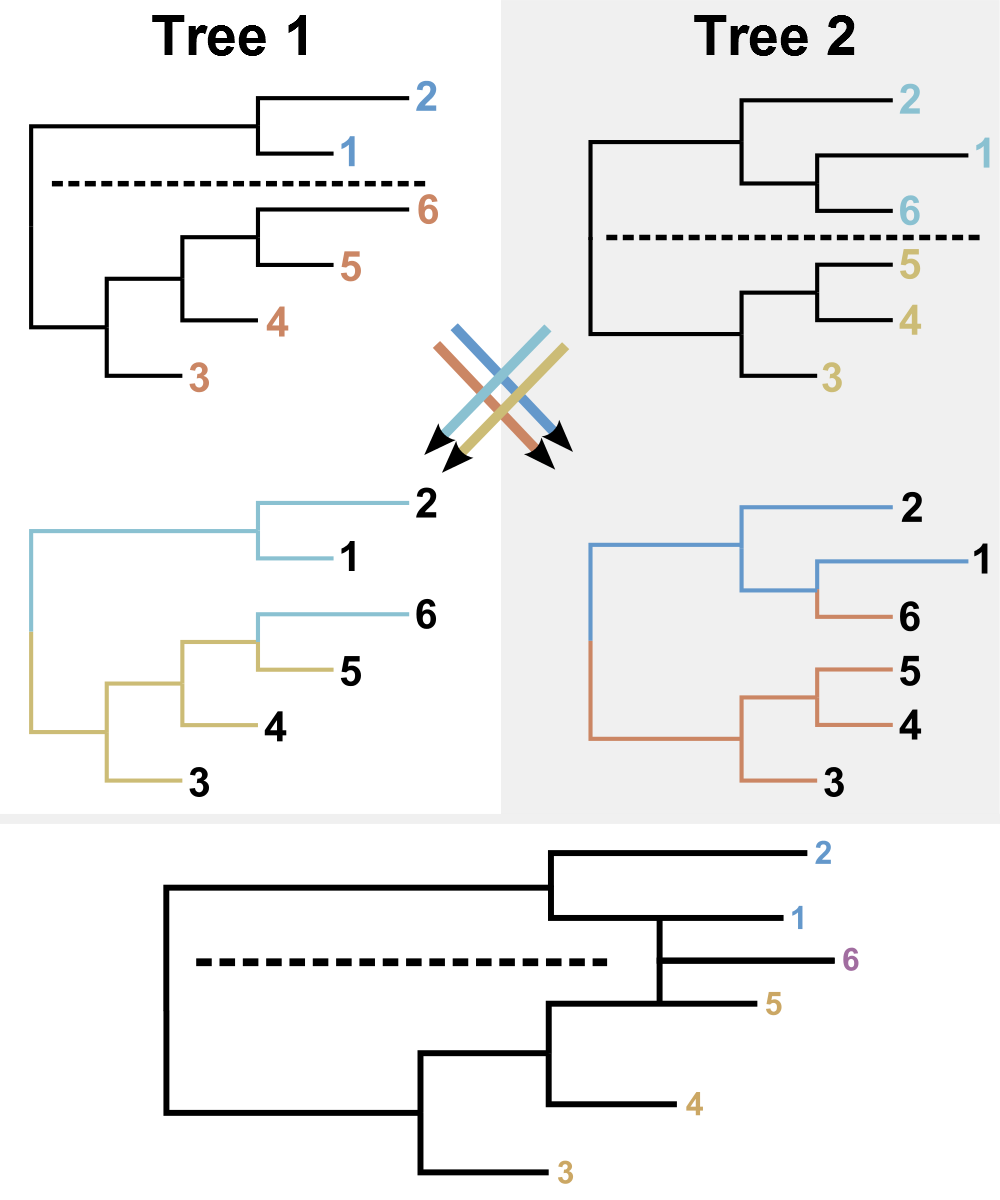
\includegraphics[width=0.45\textwidth]{figures/TreeFigure2}
	\caption{\textbf{Schematic analysis of reassortment patterns.}
	A) We begin by assigning sequences falling on either side of a specified bifurcation within each segment tree to different lineages, in this case, the Victoria and Yamagata bifurcation that occurred in the early 1980s.
	B) We then transfer lineage labels from one tree to the same tips in another tree.
	Label switches thus indicate reassortment events that combine lineages falling on different sides of the Vic/Yam bifurcation.
	C) A reassortment graph depiction shows that tip number 6 is determined to be a reassortant based on B).
	}
	\label{methodFig}
\end{figure}

\section*{Methods}
We compiled a dataset of 452 complete influenza B genomes from GISAID \cite{GISAID} dating from 1984 to 2012 (accession numbers and laboratory acknowledgements can be found in supplementary information).
The longest protein coding region of each segment was extracted and used for all further analyses.
We thus assume that homologous recombination has not taken place and that the evolutionary history of the whole segment can be inferred from the longest coding sequence in the segment.
To date there has been little evidence of homologous recombination in influenza viruses \cite{chare2003,boni2008,han2010}.
The segments of each strain were assigned to either Vic or Yam lineage by making maximum likelihood trees of each segment using PhyML \cite{guindon2003} and identifying whether the isolate was more closely related to B/Victoria/2/87 or B/Yamagata/16/88 sequences in that segment, with the exception of the NS segment (B/Victoria/2/87 was a reassortant and possessed a Yam lineage NS \cite{lindstrom1999}), where B/Czechoslovakia/69/1990 was considered as being representative of Victoria lineage.
Each strain was thus assigned 8 lineages depending on the combination of lineages from which their genomes were derived, for example all segments except for NS in strain B/Victoria/2/87 belong to Vic lineage and can thus be represented as V,V,V,V,V,V,V,Y. 

We also downloaded all available sequences of influenza B isolates sampled 1984--2013 from GISAID for which PB1, PB2 and HA segments were sequenced.
This comprised a dataset of 1433 isolates in total which became available only after the primary analyses were performed using the smaller dataset and had too many sequences to analyze using the methods described later. 
Neighbor-joining trees \cite{saitou1987} of PB1, PB2 and HA segments were made and each sequence assigned to a lineage based on grouping with either B/Victoria/2/87 or B/Yamagata/16/88 sequences, as before.
Isolates which were not assigned entirely to either the Vic or the Yam lineage across PB1, PB2 and HA segments were extracted and identified as PB1-PB2-HA reassortants.

Temporally-calibrated phylogenies were recovered for each segment using the Markov chain Monte Carlo (MCMC) methods in the BEAST software package \cite{drummond2012}.
Here, we modeled the substitution process using the HKY model of nucleotide substitution \cite{hky1985}, with separate transition models for each of the 3 codon partitions, and additionally estimate realized synonymous and non-synonymous substitution counts \cite{obrien2009}.
We used a flexible Bayesian skyride demographic model \cite{minin2008}.
We accounted for incomplete sampling dates for 94 sequences (of which 93 had only year and 1 had only year and month of isolation) whereby tip date is estimated as a latent variable in the MCMC integration.

We ran 3 independent MCMC chains, each with 200 million states, sampled every 20,000 steps and discarded the first 10\% of the MCMC states as burn-in.
After assessing convergence of all 3 MCMC chains by visual inspection using Tracer \cite{tracer}, we combined samples across chains to give a total of 27,000 samples from the posterior distribution of trees.
Maximum clade credibility trees of all 8 influenza B segments is shown in Figure \ref{genomeGrid}.

Every sequence was assigned 7 discrete traits in BEAUti corresponding to the lineages of all other segments with which a strain was isolated \textit{e.g.} PB1 tree had PB2, PA, HA, NP, NA, MP and NS as traits and V or Y as trait values.
We inferred the ancestral state of lineages in each segment by modelling transitions between these discrete states using an asymmetric transition matrix \cite{lemey2009} with Bayesian stochastic search variable selection (BSSVS) to estimate significant rates. Because the posterior set of trees for a single segment has branches labelled with the inferred lineage in the remaining 7 segments, we can detect inter-lineage reassortments between pairs of segments by observing state transitions, i.e.\ Yam to Vic or Vic to Yam (see Figure \ref{methodFig}). 
In addition, by reconstructing the ancestral state of all other genomic segments jointly we can infer co-reassortment events when more than one trait transition occurs on the same node in a tree.

\subsection*{Measures of diversity}
We inferred the diversity of each segment at a single point in time by estimating the date of the most recent common ancestor of all branches at yearly intervals, which places an upper bound on the maximum amount of diversity existing at each time period.
A version of this lineage turnover metric has previously been used to investigate the tempo and strength of selection in influenza A viruses during seasonal circulation \cite{bedford2011}.
In addition, we calculated mean pairwise time of most recent common ancestor (TMRCA) between branches labelled as Vic and Yam for PB1, PB2 and HA.
This gave us a measure of how much a particular segment reassorts with respect to Vic and Yam lineages of PB1, PB2 and HA segments.
If Vic and Yam lineages of PB1, PB2 and HA segments were to be considered as being separate populations this measure would be equivalent to `between population' diversity.

We also calculated the total amount of evolutionary time spent by each segment with entirely Vic, entirely Yam or mixed lineage PB1, PB2 and HA segments.
We do this by summing the branch lengths in each tree under 3 (2 in the case of PB1, PB2 and HA trees) different lineage combinations of the PB1, PB2 and HA segments: PB1-PB2-HA derived entirely from Yamagata lineage, PB1-PB2-HA entirely derived from Victoria lineage and PB1-PB2-HA derived from a mixture of the two lineages.
This gives a measure of how successful, over long periods of time, each particular PB1-PB2-HA constellation has been.

\subsection*{Tree to tree similarities}
We subsampled our combined posterior distribution of trees to give a total of 2700 trees.
Pairwise comparisons between each pair of segments were performed by comparing individual pairs of sampled trees.

We express the similarity of two trees by comparing the means of the distribution of TMRCA differences (which we refer to as $\Delta$TMRCA) between pairs of tips in the two trees.
In comparing TMRCAs of trees A and B we calculate
\begin{equation}
\Delta(A_i, B_i) = \frac{f(A_i, A_i') + f(B_i, B_i')}{2 \, f(A_i, B_i)},
\end{equation}
where $f(A_i, B_i) = \frac{1}{n}\sum_{j=1}^n |g(A_{ij}, B_{ij})|$ and $|g(A_{ij},B_{ij})|$ is the absolute difference in TMRCA of a pair of tips $j$, where the pair is drawn from the \textit{i}th posterior sample of tree A and the \textit{i}th posterior sample of tree B.
Additionally, $f(A_i,A'_i)$ is calculated from the \textit{i}th posterior sample of tree A and \textit{i}th posterior sample of an independent analysis of tree A (which we refer to as A'), to control for variability in tree topology stability over the course of the MCMC chain caused by differences in alignment lengths used to produce the trees.
We had 3 replicate analyses of each segment and in order to calculate $f(A_i,A'_i)$ we used analyses numbered 1, 2 and 3 as A and analyses numbered 2, 3 and 1 as A', in that order.

Calculating $\Delta(A_i, B_i)$ for each MCMC state provides us with a posterior distribution of this parameter allowing  specific hypotheses regarding similarities between the trees of different segments to be tested.
Our approach exploits the branch scaling used by BEAST \cite{drummond2012}, since the trees are scaled in absolute time and insensitive to variation in nucleotide substitution rates between segments, allowing for direct comparisons between TMRCAs in different trees.
Our $\Delta$TMRCA statistic is an extension of patristic distance methods and has previously been used to tackle a wide variety of problems, as phylogenetic distance in predicting viral titer in \textit{Drosophila} infected with viruses from closely related species \cite{longdon2011} and as \textit{$\Delta$t} to assess temporal incongruence in a phylogenetic tree of amphibian species induced by using different calibrations \cite{ruane2011}.

Subtree prune and regraft (SPR) distances between phylogenetic trees are an approximate measure of the numbers of reassortment or recombination events.
Exact SPR distances are difficult to compute, as they depend on the SPR distance itself and are impractical to compute for posterior distributions of trees except for the most similar trees.
We calculated approximate SPR distances \cite{whidden2009,whidden2010,whidden2013} to quantify the numbers of reassortments that have taken place between all pairs of segments.
Approximate SPR distances were normalized using the procedure described above, where $f(A_i, A_i')$, $f(B_i, B_i')$ and $f(A_i, B_i)$ are approximate SPR distances between \textit{i}th posterior samples from trees A, B and independent analyses thereof (A' and B').

\subsection*{Linkage disequilibrium across the influenza B genome}
We estimated linkage disequilibrium (LD) between amino acid sites across the longest proteins encoded by each segment of the influenza B virus genome.
To quantify LD we used the $\chi^{2}_{df}$ statistic \cite{zhao2005}, as it is equal to the widely used \textit{r$^{2}$} LD statistic at biallelic loci, but also quantifies LD when there are more than two alleles per locus.
LD was estimated only at loci where each nucleotide or amino acid allele was represented by at least two isolates.
We ignored gaps in the alignment and did not consider them as polymorphisms.
We also calculated mean LD for all pairs of segments to quantify the overall association between them.
Linkage disequilibrium was not estimated for the larger PB1, PB2 and HA dataset, because it lacked sequences from the rest of the influenza B genome and thus would have failed to put LD between PB1, PB2 and HA proteins into a genome-wide perspective.

\section*{Results}

\subsection*{Phylogenetic analyses reveal maintenance of diversity and co-assortment of PB1, PB2 and HA gene segments}
The differentiation into Vic and Yam lineages can be seen in all segments \cite{chen2008} (see Figure \ref{genomeGrid}).
Following the split of the two lineages, each segment can be assigned to either Vic or Yam lineage and inter-lineage reassortment events have yielded mixed-lineage genome constellations.
Some segment lineages associated with mixed-lineage genomes have become fixed in the influenza B virus population, i.e.\ became the `trunk' of the phylogenetic tree of a segment.
Overall, we see many old bifurcations within the trees of all segments.
Many of these correspond to reassortment events involving the PB1, PB2 and HA segments of Vic and Yam lineages, highlighting the role reassortment plays in the long-term evolution of influenza B viruses.

By quantifying patterns of ancestry across contemporaneous viruses for each segment, it is clear that the PA, NP, NA, MP and NS segments have undergone periodic losses of diversity, while the PB1, PB2 and HA segments have maintained diversity up to the present (Figure \ref{tmrcaOT}).
The PB1, PB2 and HA segments maintain a common ancestor in $\sim$1983 up to the present and thus accumulate genetic diversity since the split of those segments into Vic and Yam lineages, while other segments often lose diversity with ancestors to present day viruses appearing between $\sim$1991 and $\sim$1999.

\begin{figure}[h]
	\centering		
	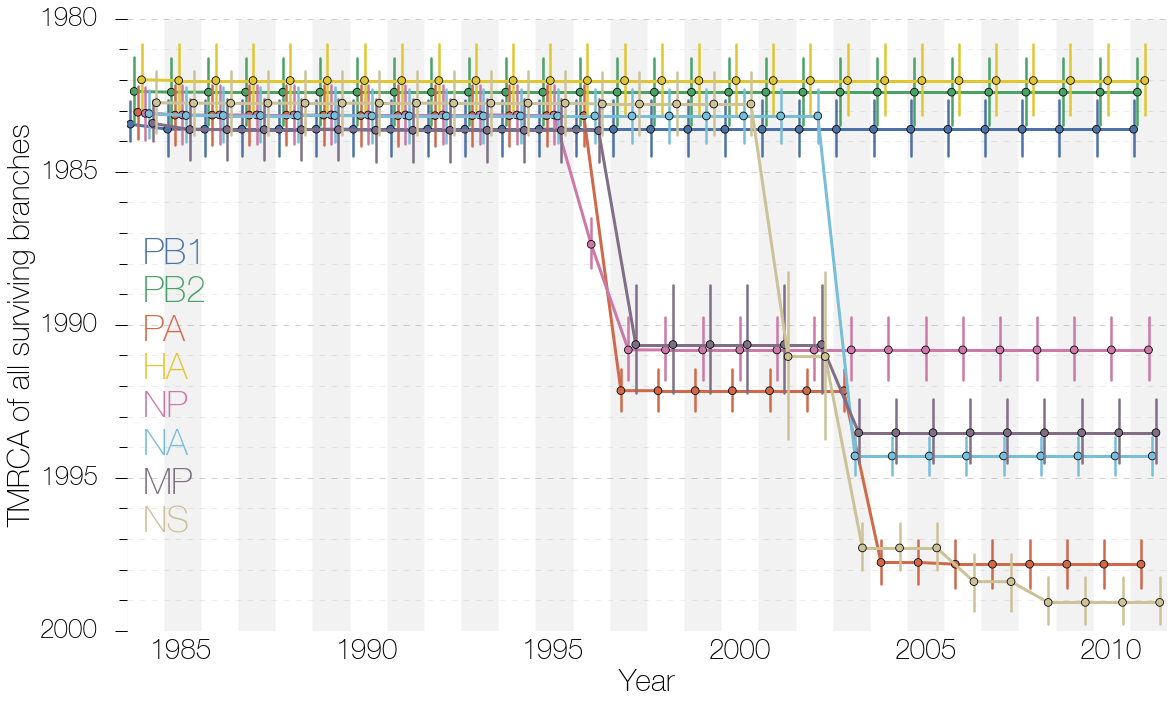
\includegraphics[width=0.75\textwidth]{figures/InfB_tmrcaOT_lines.png}
	\caption{\textbf{Oldest TMRCA of all surviving branches over time.}
PA, NP, NA, MP and NS segments of influenza B viruses show periodic losses of diversity, indicating lineage turnover.
PB1, PB2 and HA segments, on the other hand, maintain the diversity dating back to the initial split of Vic and Yam lineages.
Each point is the TMRCA of all surviving lineages existing at each time slice through the tree and vertical lines indicating uncertainty are 95\% highest posterior densities (HPDs).}
	\label{tmrcaOT}
\end{figure}

By measuring mean pairwise diversity between branches in each tree that were assigned either a Vic or Yam label in other segments, we look for reductions in between lineage diversity, which indicate that an inter-lineage reassortment event has taken place (Figure \ref{betweenDiversity}).
Because we are taking the mean of pairwise comparisons, this method gives a quantitative measure of diversity of panmixis between Victoria and Yamagata lineages in two trees, although care should be taken when interpreting the statistic, as it does not correspond to any real TMRCAs in the tree.
We focus only on PB1, PB2 and HA lineage labels, since all other segments have fixed either the Vic or the Yam lineage.
Losses of diversity (represented by more recent mean pairwise TMRCAs between Vic and Yam labels) in Figure \ref{betweenDiversity} in all 8 segment trees indicate that every segment has reassorted with respect to the Victoria and Yamagata lineages of PB1, PB2 and HA segments.
However, we also see that PB1, PB2 and HA labels show reciprocal preservation of diversity after 1997.
This suggests that no reassortment events have taken place between Victoria and Yamagata lineages of PB1, PB2 and HA segments.
After 1997 in PB1, PB2 and HA trees PB1, PB2 and HA traits only `meet' at the root.
In a time period close to the initial split of Vic and Yam lineages (1986--1996) we see reduced diversity between Vic and Yam labels of PB1, PB2 and HA segments.
These reductions in diversity represent small clades with reassortant PB1-PB2-HA constellations, which go extinct by 1997.
We also observe that the assignment of Vic or Yam lineages of PB1, PB2 and HA segments to branches of other segment trees is very similar and often identical.
This results in PB1, PB2 and HA lineage labels switching between Vic and Yam simultaneously in all trees after 1997, suggesting co-reassortment of Vic and Yam lineages of PB1, PB2 and HA segments. 

\begin{figure}[h]
	\centering		
	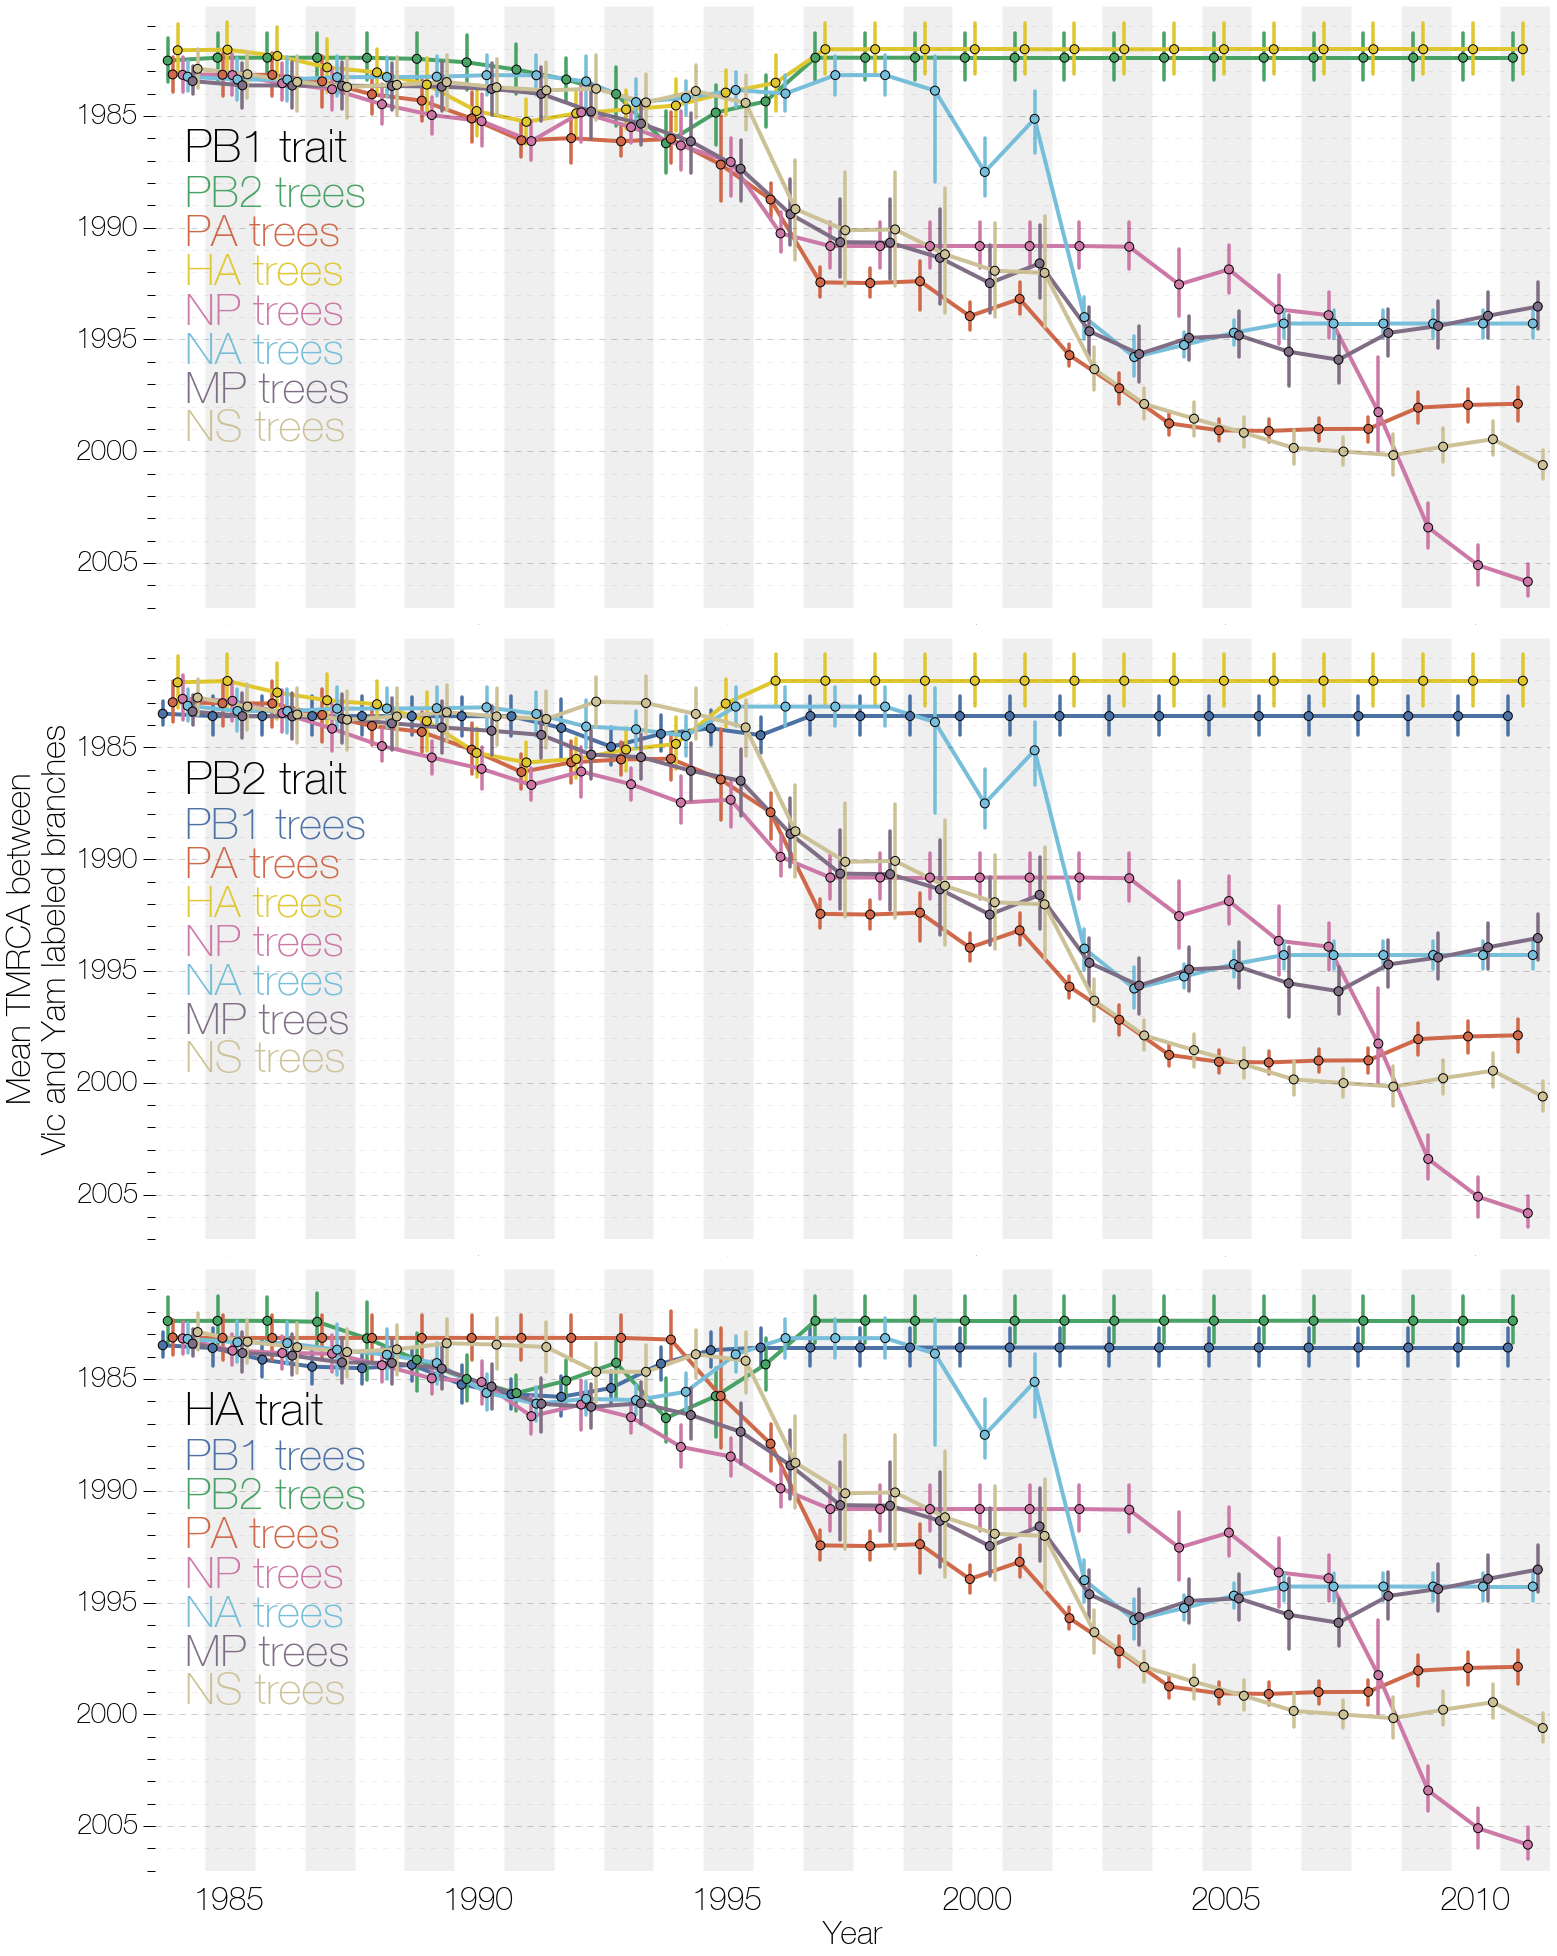
\includegraphics[width=0.75\textwidth]{figures/InfB_betweenDiversity.png}
	\caption{\textbf{Mean pairwise TMRCA between Vic and Yam branches under PB1, PB2 and HA label sets.}
PB1, PB2 and HA segment labels indicate that these segments show reciprocal preservation of diversity, which dates back to the split of Vic and Yam lineages.
All other segments show increasingly more recent TMRCAs between branches labelled as Vic and Yam in PB1, PB2 and HA label sets.
All vertical lines indicating uncertainty are 95\% highest posterior densities (HPDs).}
	\label{betweenDiversity}
\end{figure}

By plotting the ratios of sequences assigned to either Vic or Yam lineage in each segment (Figure \ref{lineageRatiosOverTime}) it is evident that losses of diversity in the PA, NP, NA, MP and NS segments are related to the repeated fixation of either the Vic or the Yam lineage.
These losses of diversity correspond to fixation of the Vic lineage in NS and fixation of the Yam lineage in PA, NP, NA and MP.
Similarly, the lack of reassortment between Vic and Yam lineages and maintenance of diversity of PB1, PB2 and HA can be seen (Figure \ref{lineageRatiosOverTime}), where the two lineages have been isolated at a ratio close to 50\% over long periods of time.
On a year-to-year basis, however, the ratios for Vic and Yam lineage PB1, PB2 and HA can fluctuate dramatically suggesting that one lineage may predominate within a given season, consistent with surveillance data \cite{reed2012}.

\begin{figure}[h]
	\centering	
	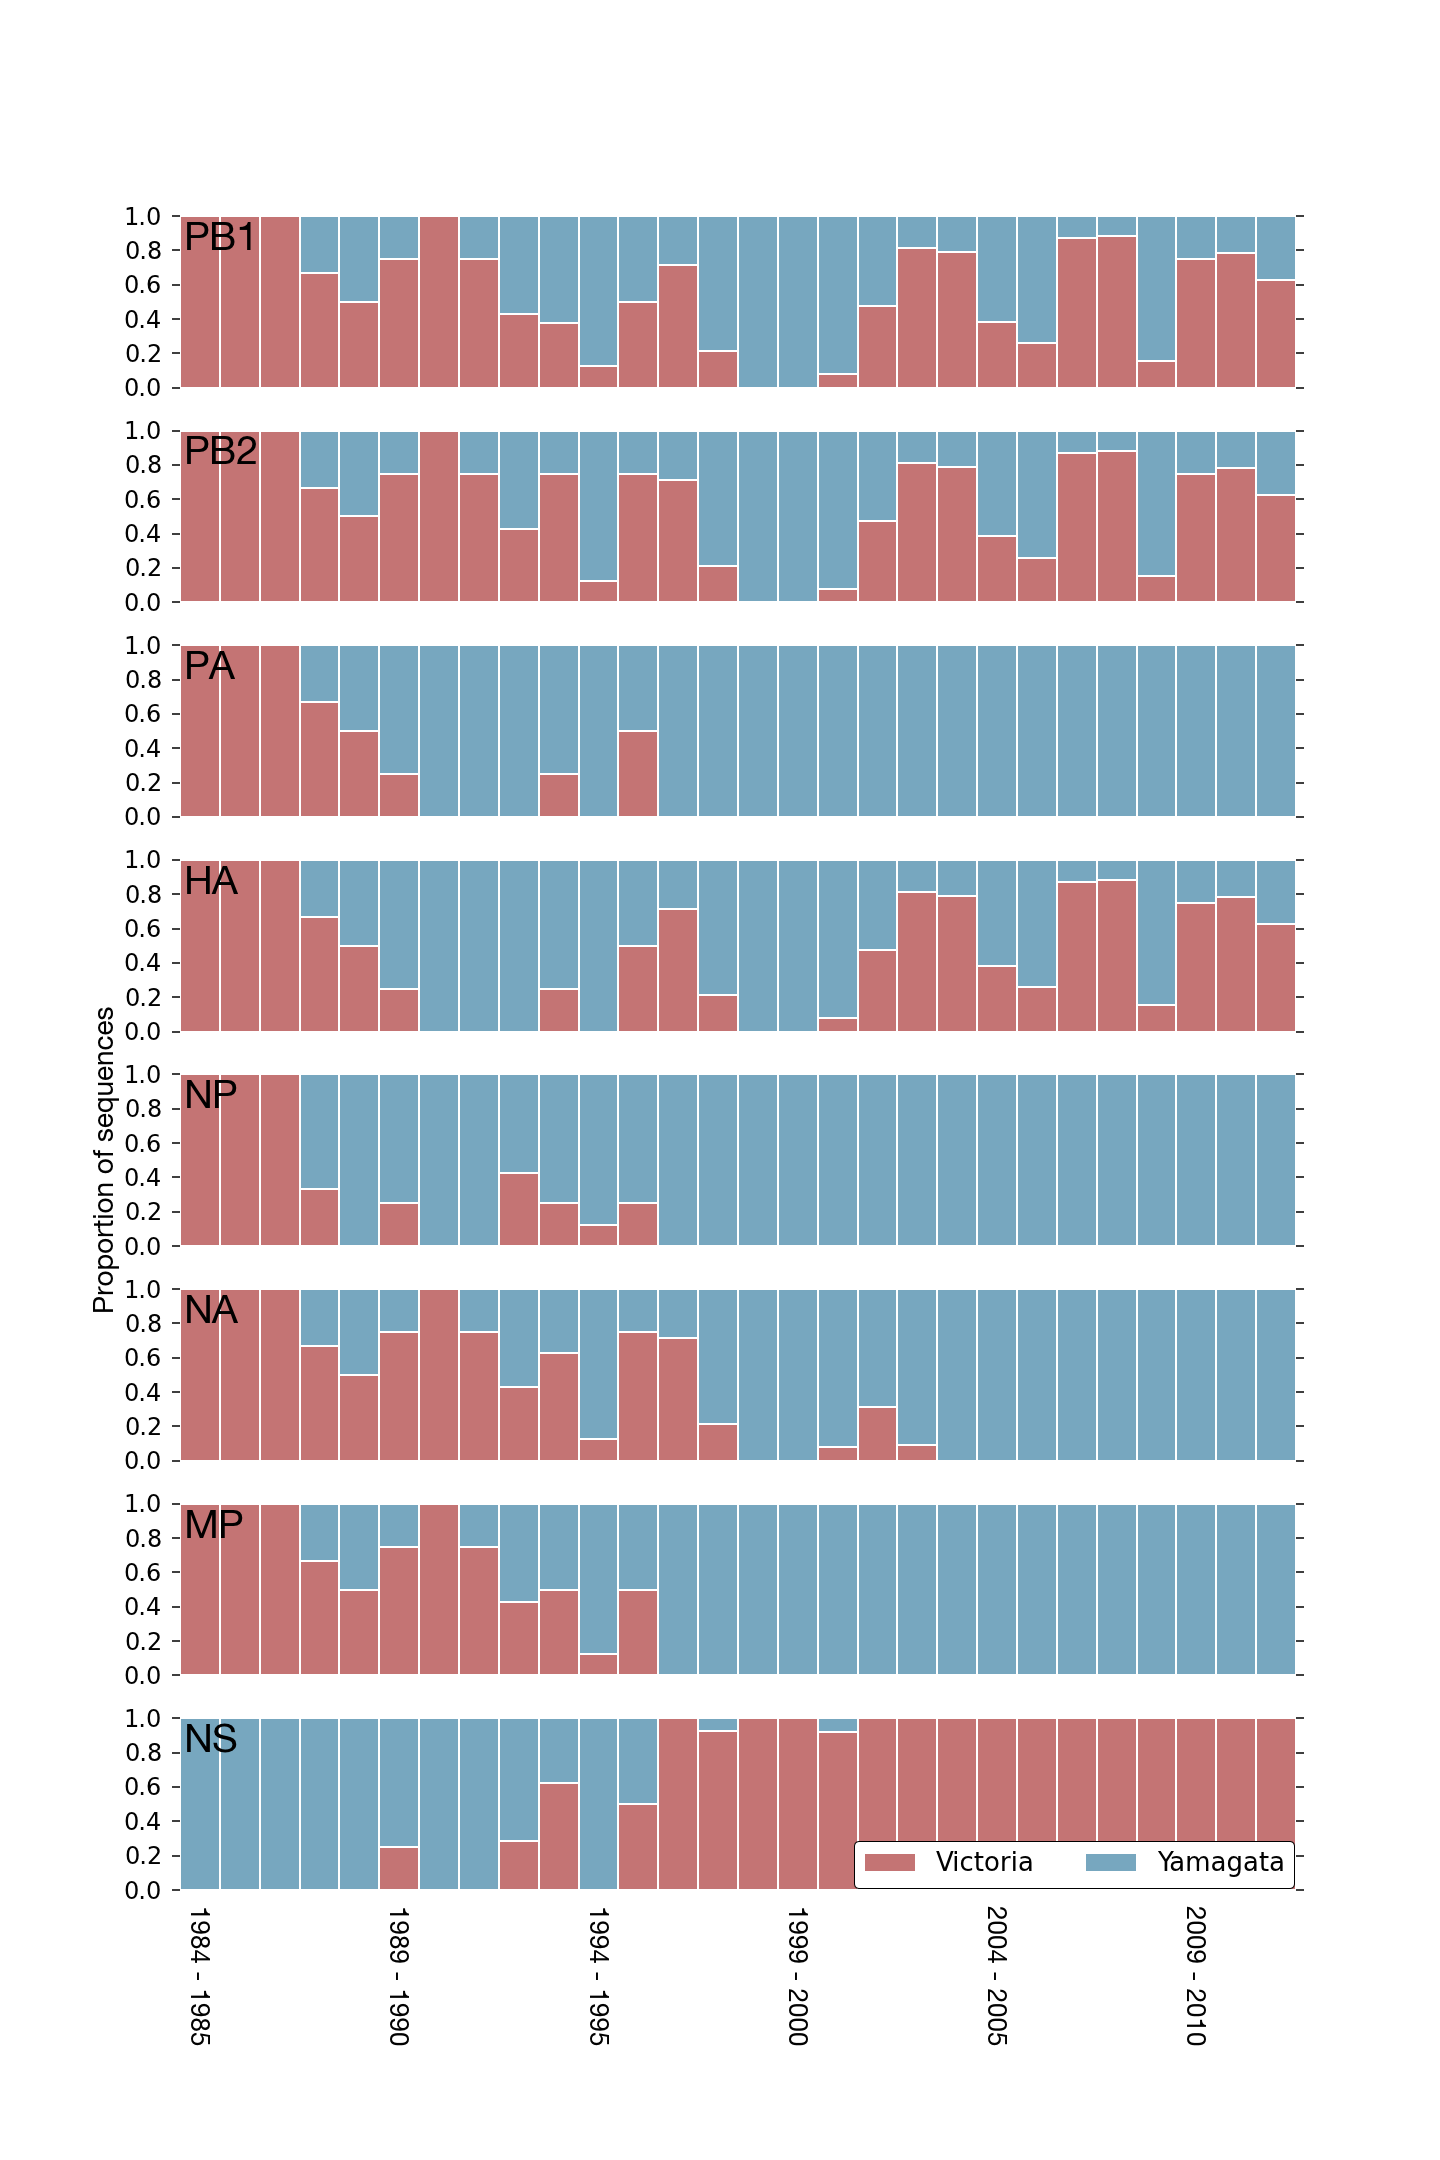
\includegraphics[width=0.65\textwidth]	{figures/InfB_LineageRatiosOverTime.png}
	\caption{\textbf{Ratio of lineages in the dataset.}
The ratio of sequences that derive from the original Victoria clade (orange) to sequences that derive from the Yamagata clade (grey) in each segment over time.
Yamagata lineage PA, NP, NA and MP segments and Victoria lineage NS segment eventually become fixed in the influenza B population.
PB1, PB2 and HA segments maintain separate Victoria and Yamagata lineages.}
	\label{lineageRatiosOverTime}
\end{figure}

We reconstructed reassortment events that were detected by using lineage labels.
Figure \ref{railroadPlot} focuses only on inter-lineage reassortments that have occured after 1990.
We identify 5 major reassortant genome constellations (given in order PB1-PB2-PA-HA-NP-NA-MP-NS) circulating 1992 -- 2011: B/Alaska/12/1996-like (YYYYYYYV), B/Nanchang/2/1997-like (VVYVYVYV), B/Iowa/03/2002-like (VVYVYYYV), B/California/NHRC0001/2006-like (VVYVYYYV) and B/Brisbane/33/2008-like (VVYVYYYV) in Figure \ref{railroadPlot}.
Of these 5 constellations 4 (B/Nanchang/2/1997-like, B/Iowa/03/2002-like, B/California/NHRC0001/2006-like and B/Brisbane/33/2008-like) are derived from introgression of Yamagata lineage segments into Victoria lineage PB1-PB2-HA background, with only 1 (B/Alaska/12/1996-like) resulting from introgression of Victoria lineage NS segment into an entirely Yamagata lineage derived background.
All 5 inter-lineage reassortment events described here are marked by the preservation of either entirely Victoria or Yamagata lineage derived PB1-PB2-HA segments.
Figure \ref{railroadPlot} also shows that reassorting segments appear to evolve with a considerable degree of autonomy.
For example, the NP lineage that entered a largely Victoria lineage derived genome and gave rise to the B/Nanchang/2/1997-like isolates continued circulating until 2010, even though other segments it reassorted with in 1995 -- 1996 (PA and MP) went extinct following the reassortments that led to the rise of viruses with B/Iowa/03/2002-like genome constellations.
A more extreme example is the NS segment, which in B/Iowa/03/2002-like isolates (and all subsequent Vic PB1-PB2-HA isolates) has originally been derived from the Victoria lineage that had been associated with mostly Yam lineage derived B/Alaska/12/1996-like genomes for a number of years.

\begin{figure}[h]
	\centering		
	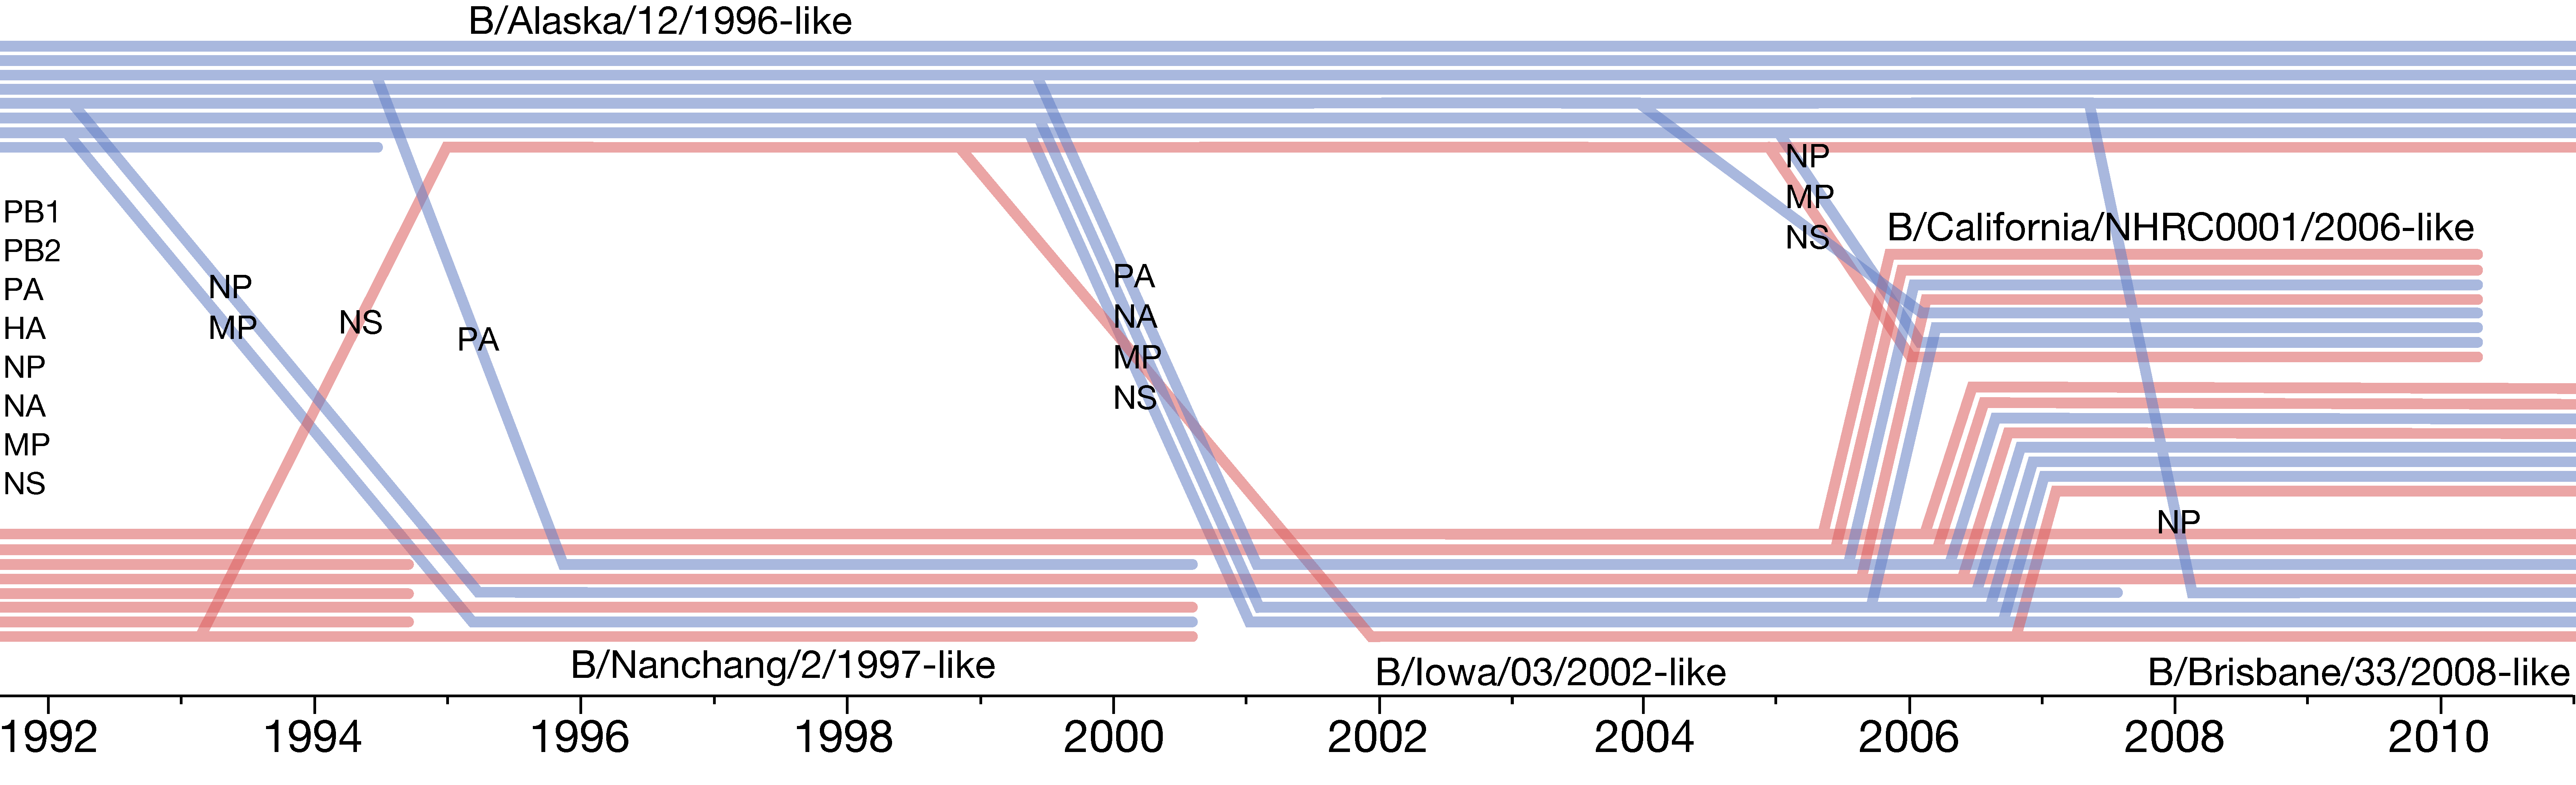
\includegraphics[width=0.95\textwidth]{figures/RailroadPlotDated.pdf}
	\caption{\textbf{Schematic plot of reconstructed reassortments between Victoria and Yamagata lineage segments of influenza B virus.}
Lineages that coassort in genomes are represented by 8 parallel lines, with lineages that derive from the original Victoria clade colored orange and lineages that derive from the original Yamagata clade colored grey.
Inter-lineage reassortment events are indicated by lines entering a different genome.
The angle of incoming lineages represents uncertainty in the timing of the event (mean date of the reassortant node and its parent node).
Lineage extinction dates are not shown accurately.}
	\label{railroadPlot}
\end{figure}

\subsection*{Recent PB1-PB2-HA constellations are entirely derived from Victoria or Yamagata lineage segments}
Figure \ref{stateTime} shows the sum of branch lengths which were labelled as having entirely Vic, entirely Yam or mixed-lineage PB1, PB2 and HA segments.
Due to lack of reassortment between Vic and Yam lineages of PB1, PB2 and HA (Figure \ref{betweenDiversity}) since 1997 all segments have spent significantly longer periods of evolutionary time with either entirely Vic-derived or entirely Yam-derived than with mixed-lineage PB1, PB2 and HA constellations (Figure \ref{stateTime}).

\begin{figure}[h]
	\centering		
	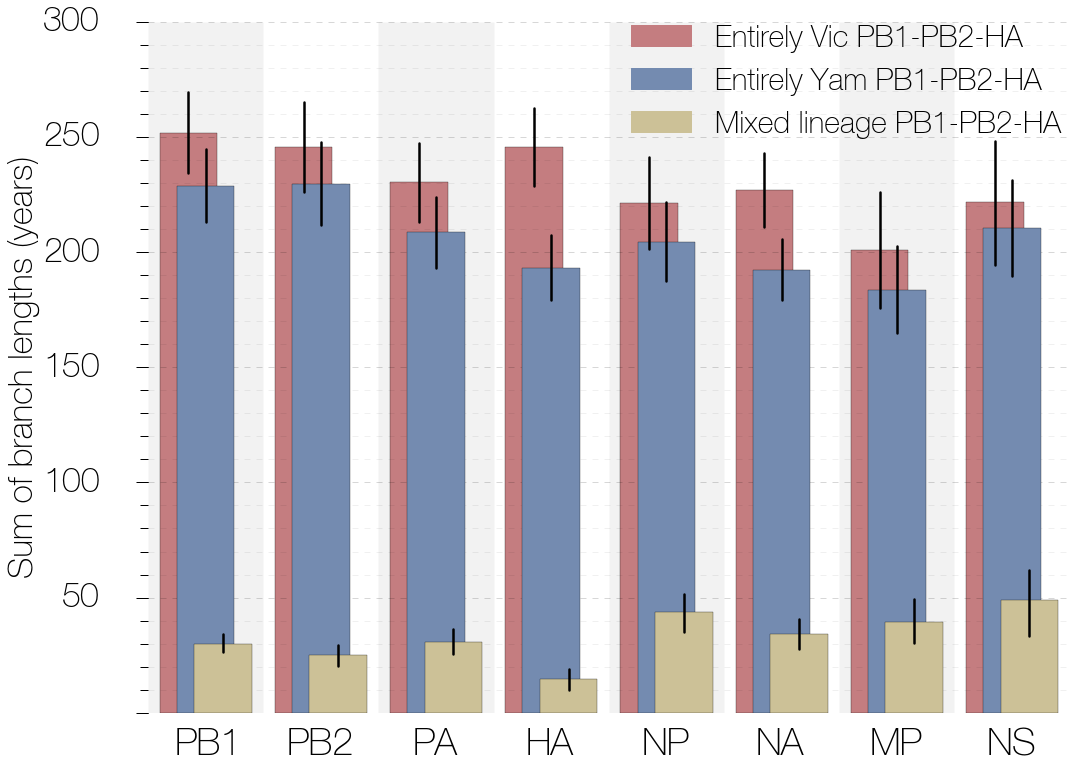
\includegraphics[width=0.65\textwidth]{figures/InfB_stateTime.png}
	\caption{\textbf{Amount of evolutionary time spent under different PB1-PB2-HA constellations.}
All segments have spent significantly more of their history with entirely Vic or entirely Yam-derived PB1-PB2-HA complexes.
All horizontal lines indicating uncertainty are 95\% highest posterior densities (HPDs).}
	\label{stateTime}
\end{figure}

We have identified 3 instances of mixed-lineage PB1-PB2-HA reassortants from the data with the following PB1-PB2-HA constellations: VVY (B/Bangkok/163/1990-like, 13 sequences isolated 1990 -- 5 Jan 1995), VYV (B/Nanchang/630/1994-like, 2 sequences isolated 1994 -- 1996) and VYY (B/New York/24/1993-like, 2 sequences isolated 8 Jan 1993 -- 1994).
An additional instance of reassortants with a YYV PB1-PB2-HA constellation (B/Waikato/6/2005-like, 16 sequences isolated 9 June -- 12 November in 2005) was discovered when investigating the larger dataset with only PB1, PB2 and HA sequences.

In all cases, PB1-PB2-HA reassortants have not persisted for prolonged periods of time and have not been fixed in the influenza B population.
In particular reassortment events combining PB1 and PB2 segments of different lineages, \textit{e.g.} B/Nanchang/630/1994-like and B/New York/24/1993-like isolates (each represented by two isolates), exhibit poor sampling and short circulation times.
In the case of B/Nanchang/630/1994-like viruses this is up to two years.
In contrast, reassortments combining PB1+2 and HA of different lineages (B/Bangkok/163/1990-like and B/Waikato/6/2005-like isolates) have more isolates and circulated for much longer periods of time in the past: up to 4 years for B/Bangkok/163/1990-like, although the more recently isolated B/Waikato/6/2005-like viruses circulated for only 5 months.

\subsection*{PB1, PB2 and HA trees experience reassortment `distance' effects}
SPR (subtree prune and regraft) distances between perfectly resolved pairs of trees would be equal to the number of reassortments that have taken place between the two trees and is a measure of tree-to-tree similarity.
Figure \ref{SPRdistances} shows approximate SPR distances between all pairs of segment trees after normalization (see Methods).
If there are biases in the way segments reassort, so that some segments tend to co-reassort more often, we expect to see small-scale similarities between phylogenetic trees of those segments.
In our case we expect SPR distances, which are proportional to the number of reassortment events that have taken place between trees, to reflect the raw (\textit{i.e} both within and between lineages) reassortment rate.

\begin{figure}[h]
	\centering		
	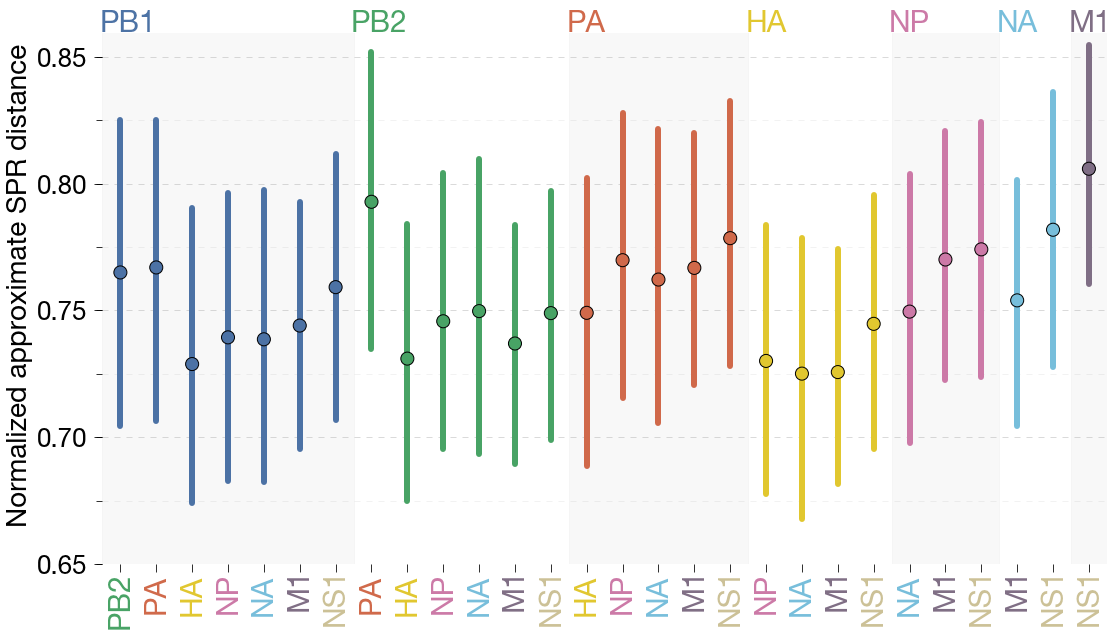
\includegraphics[width=0.65\textwidth]{figures/InfB_normalizedApproxSPR.png}
	\caption{\textbf{Normalized approximate SPR distances between pairs of segments.}
Following the normalization procedure approximate SPR distances are similar across all pairwise comparisons.
We interpret this as lack of evidence for small-scale topological similarities between trees of all segments, which we expect to arise if any two segments were being co-packaged.
All vertical lines indicating uncertainty are 95\% highest posterior densities (HPDs).}
	\label{SPRdistances}
\end{figure}

In Figure \ref{SPRdistances} the 95\% highest posterior density (HPD) intervals of normalized approximate SPR distances between pairs of segments encompass most means and occupy a relatively small range, suggesting there is no evidence of differences in the number of reassortments (or reassortment rate given as number of SPR moves per total time in both trees, see Figure \ref{NormSPR_RErate} in supplementary information) between all segments.
We note, however, that our SPR distance analysis might simply lack power.
Comparisons between independent analyses of the same segments yield distances that are comparable to distances between different segments (see Figures \ref{SPRdistancesTrees} and \ref{SPRdistancesReplicates}), suggesting that phylogenetic uncertainty is making a considerable contribution to our estimates of approximate SPR distances.
In addition, SPR distances themselves can only approximate (and underestimate) the actual numbers of reassortments.
Thus we caution against over-interpreting Figure \ref{SPRdistances}.
Although there might be concern about using approximate, rather than exact, SPR distances we do estimate exact SPR distances for a limited number of segment pairs - PB1, PB2 and HA - and find that after normalization exact and approximate SPR distances are not significantly different (see supplementary Figures \ref{NormSPR_PB1-PB2_difference}--\ref{NormSPR_PB2-HA_correlation}). 

Although we do not find evidence of differences in numbers of raw reassortments between all pairs of trees, we find support for a reassortment `distance' effect.
Figure \ref{deltaTMRCA} shows normalized mean $\Delta$TMRCA values for all pairs of trees.
Most segment pairs show very low values for this statistic, indicating considerable differences between TMRCAs of the trees being compared.
A large number of these comparisons have TMRCA differences up to 10 times larger ($\Delta$TMRCA$\approx$0.1) than TMRCA differences that occur between replicate BEAST analyses of one alignment over the course of the MCMC chain.
PB1, PB2 and HA trees, on the other hand, exhibit normalized $\Delta$TMRCA values that are much higher.
This is an indicator of TMRCA differences between trees of PB1, PB2 and HA segments which, though noisy, are occassionally very similar to uncertainty in tip-to-tip TMRCAs between replicate analyses of these segments.
Overall, it suggests that PB1, PB2 and HA lineages tend to not reassort amongst themselves unless both reassorting segments have similar TMRCAs, i.e.\ there is isolation by distance.
In addition, we see evidence of a similar reassortment `distance' effect in MP and NA trees in Figure \ref{deltaTMRCA}.
Previously, associations between MP and NA segments have been suspected in influenza A viruses (Samantha Lycett, personal communication).

\begin{figure}[h]
	\centering		
	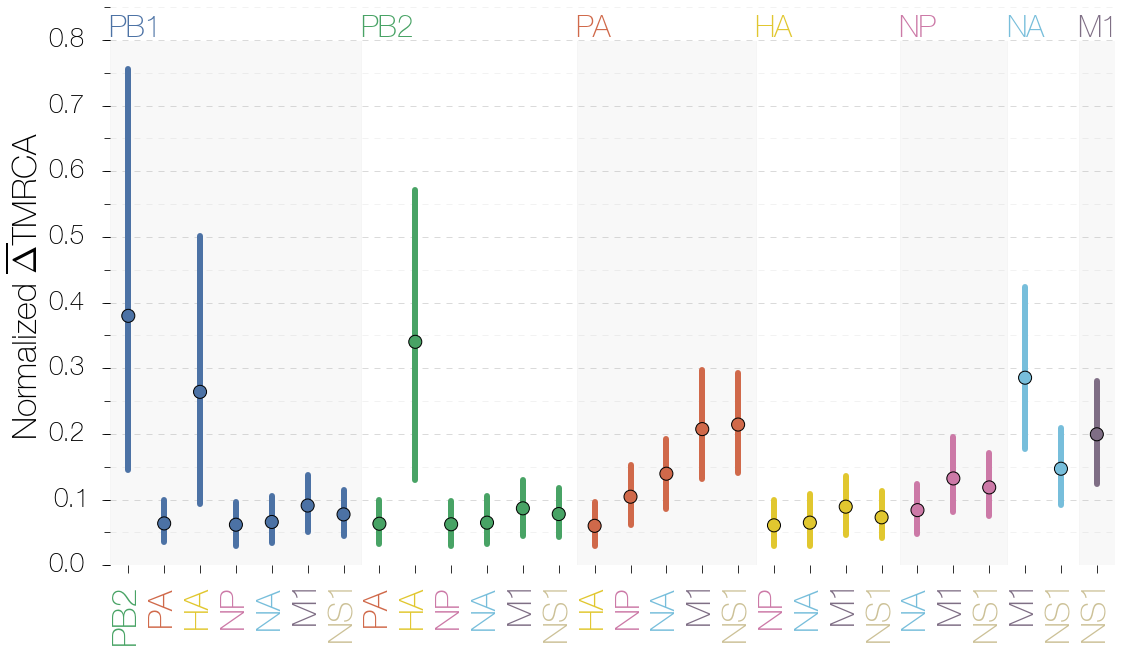
\includegraphics[width=0.65\textwidth]{figures/InfB_normalizedMuDeltaTMRCA.png}
	\caption{\textbf{Normalized mean $\Delta$TMRCA statistics between pairs of segments.}
PB1, PB2 and HA trees exhibit reciprocally highly similar TMRCAs, unlike most other pairwise comparisons.
All vertical lines indicating uncertainty are 95\% highest posterior densities (HPDs).}
	\label{deltaTMRCA}
\end{figure}

\subsection*{Linkage disequilibrium analysis confirms phylogenetic findings}
Linkage disequilibrium (LD) is a measure of association between alleles at different polymorphic loci within a population.
To estimate LD no other information, except for alleles at polymorphic amino acid sites in the dataset, is required.
Although not an independent validation of association between PB1, PB2 and HA segments, linkage disequilibrium analyses show that Victoria and Yamagata lineages of these segments have accumulated lineage-specific amino acid substitutions.
In Figure \ref{segmentLD} the signature of Vic and Yam lineage-specific substitutions is greater mean $\chi^{2}_{df}$ between PB1, PB2 and HA amino acid sites than any other pair of proteins.
In some cases this value exceeds the estimated mean LD of amino acid sites within the same protein (\textit{e.g.} PB1 and HA have higher mean LD than mean LD when PB1 is compared against itself).

\begin{figure}[h]
	\centering	
	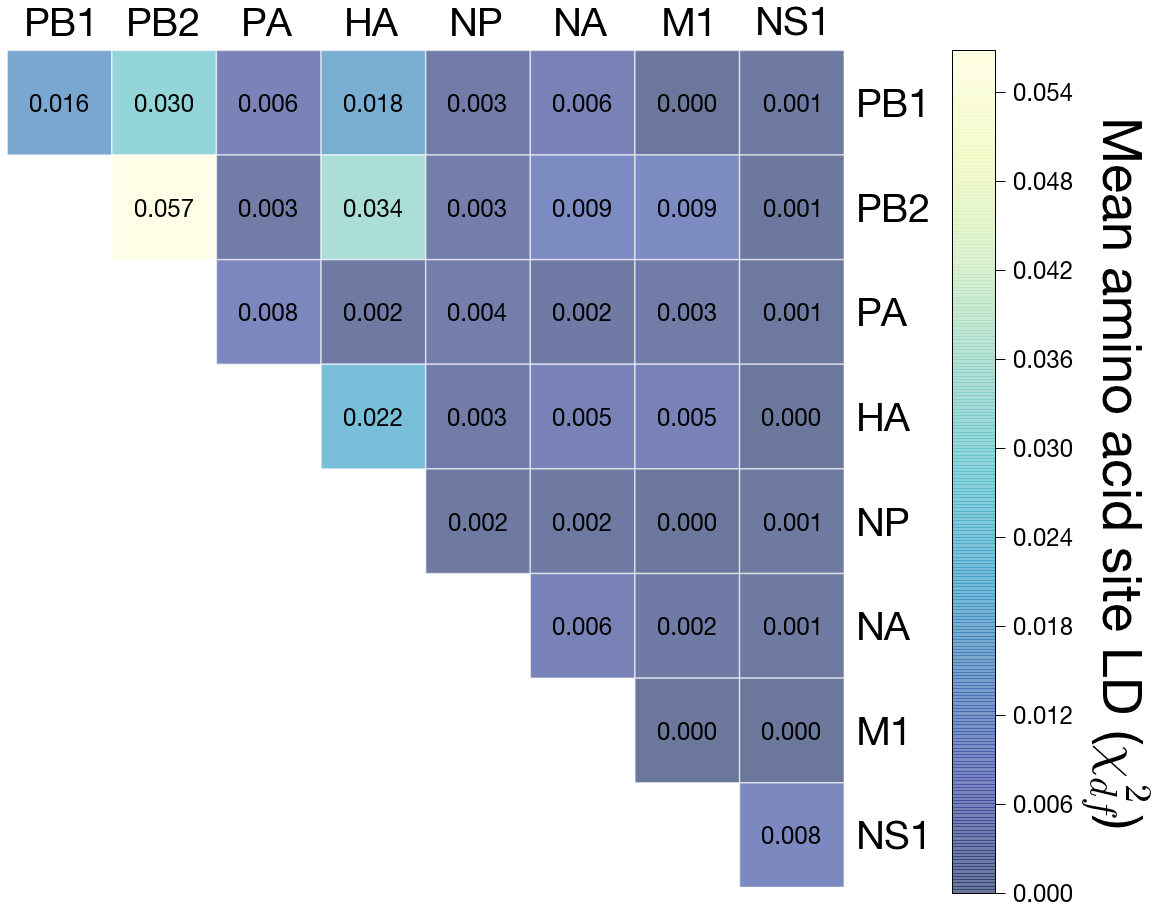
\includegraphics[width=0.65\textwidth]{figures/InfB_aaMeanLD.png}
	\caption{\textbf{LD comparison between influenza B proteins.}
Pairwise comparisons of linkage disequilibrium between amino acid sites on influenza B proteins.
PB1, PB2 and HA proteins exhibit high mean amino acid LD between themselves.
This is evidence of a considerable number of co-assorting alleles within these proteins.}
	\label{segmentLD}
\end{figure}

Of the amino acid sites that exhibit high LD on PB1, PB2 and HA proteins, there are 5 sites on PB1, 8 on PB2 and 13 on HA proteins which form a network of sites exhibiting reciprocally high LD (see Figures \ref{ChiGenome} and \ref{ChiCore} in supplementary information).
These sites define the split between Vic and Yam lineages within PB1, PB2 and HA segments.
In addition, there are sites on PB1, PB2 and HA proteins which also show high, albeit smaller, LD which correspond to sites which have undergone amino acid replacements some time after the Vic/Yam split.

\section*{Discussion}

\subsection*{Evidence of a co-adapted PB1-PB2-HA gene complex}
In this paper we show that the PB1, PB2 and HA segments of influenza B viruses are the only ones that have continuously maintained separate Vic and Yam lineages, while other segments have fixed either Vic or Yam lineages (Figures \ref{tmrcaOT}--\ref{railroadPlot}).
Evidence suggests that this is a result of prolonged lack of reassortment between Vic and Yam lineages in PB1, PB2 and HA (Figure \ref{betweenDiversity}) which possess co-assorting sequences detectable as high linkage disequilibrium (Figure \ref{segmentLD}).
We propose that this pattern of non-reassortment is due to the action of selection and not simply biased reassortment.
Figures \ref{SPRdistances} and \ref{deltaTMRCA} show that despite all pairs of segments having the same reassortment frequency, suggesting there is no bias in segment packaging, PB1, PB2 and HA segments exhibit much lower reassortment `distances'.

Reassortment `distances' represent the temporal separation of reassorting branches and suggests that reassortments between PB1, PB2 and HA segments tend to combine branches that have relatively recently been part of the same genome, i.e.\ that have shared a recent common virion.
In addition, most strains with mixed-lineage PB1-PB2-HA complexes occured in the early years of the Vic--Yam split, when the two lineages were much more similar at the nucleotide and amino acid levels.
The most recent influenza B viruses with B/Waikato/6/2005-like genome constellations possessed mixed-lineage PB1-PB2-HA complexes and circulated for only 5 months before presumably going extinct.
We suggest that the preservation of two PB1-PB2-HA complex lineages is similar to genomic speciation islands, where small numbers of genes resist being homogenized through gene flow \cite{turner2005}.

\subsection*{Causes of co-dependence between PB1-PB2-HA}
Previous studies have investigated possible co-dependence patterns between segments of influenza B viruses, by focusing on segments which would be expected to be co-adapted, \textit{e.g.} PB1-PB2-PA and HA-NA \cite{mccullers2004}.
Though it would be easy to explain co-adaptation between these segments by referring to their functional roles \textit{e.g.} PB1-PB2-PA form the polymerase heterotrimer and HA-NA have antagonistic activities, our findings suggest a counter-intuitive relationship between PB1, PB2 and HA segments.

It is clear that PB1-PB2-HA segments of Vic and Yam lineages do not preferentially reassort together: there have been at least 4 sampled mixed-lineage PB1-PB2-HA complex constellations which did not become fixed in the population and our estimates of the number of reassortments do not differ significantly between all segments (Figure \ref{SPRdistances}).
The latter is in line with recent experiments in influenza A that have shown that reassortment between segments differing by a single synonymous difference is highly efficient \cite{marshall2013}.
In the absence of clear functional explanations for why PB1, PB2 and HA should be co-adapted we offer several alternatives.

It is perhaps easiest to explain co-dependence between PB1 and PB2 segments based on their functions as part of the influenza RNA-dependent RNA polymerase (RdRp) heterotrimer.
Indeed, trees of PB1 and PB2 segments exhibit high similarity in tip--tip TMRCAs (Figure \ref{deltaTMRCA}), suggesting highly similar TMRCAs.
In addition, PB1--PB2 reassortants are the rarest and least persistent amongst mixed-lineage PB1-PB2-HA strains and have not been isolated since 1996.

Explaining the co-dependence of PB1+2 and HA segments is more difficult.
Many studies have noted a possible link between the HA, NA and PB1 segments of influenza A viruses \cite{bergeron2010,fulvini2011}.
Early influenza A vaccines used to be derived by infecting chicken eggs with an egg-adapted strain and a seasonal human isolate in the presence of antisera raised against the HA and NA proteins of the egg-adapted strain, thus selecting for reassortants which were egg-adapted, i.e.\ had internal segments derived from the egg-adapted strain, but possessed the HA and NA segments of the seasonal strain.
However, in addition to producing reassortants with HA-NA derived from the seasonal strain, as intended, the second most frequent class of reassortants produced using this methods were those with PB1, HA and NA derived from seasonal strains \cite{bergeron2010,fulvini2011}.

Recent experiments have suggested that the presence or absence of a `foreign' PB1 segment can have dramatic effects on HA concentration on the surface of virions and total virion production \cite{cobbin2013}.
Additional evidence for a relationship between PB1 and HA segments in influenza A viruses is given by previous influenza pandemics, which were caused by avian-human influenza A virus reassortants.
It has been established that at least for the 1957 and the 1968 influenza pandemics, caused by A/H2N2 and A/H3N2 subtypes, respectively, the viruses responsible were reassortants possessing PB1 and HA segments derived from avian influenza A viruses \cite{kawaoka1989}.
However, there have also been reassortant influenza A viruses circulating for prolonged periods of time in humans that did have disparate PB1 and HA segments, \textit{e.g.} H1N2 outbreaks in 2001 \cite{gregory2002} and H1N1/09 in 2009 \cite{smith2009}.

Another possibility is the action of balancing selection in preserving the diversity in one segment, whilst the other segments hitchhike along.
A good candidate for this would be HA, as it is now the sole bearer of substantial antigenic diversity within the influenza B population, as the Vic lineage NA segment went extinct in 2002 (Figures \ref{tmrcaOT}, \ref{lineageRatiosOverTime} and \ref{railroadPlot})).
We find this scenario unlikely: if PB1+2 segments were hitchhiking with the HA segment stochastically we would expect to see more PB1+2 versus HA reassortants and fixation of Vic or Yam lineage PB1+2 segments in the influenza B population.
Our main dataset comprising 452 complete influenza B virus genomes has one instance of these kinds of reassortants characterised by B/Bangkok/163/1990-like genome constellations.
The larger dataset with 1433 PB1, PB2 and HA sequences has an additional example of this: isolates with B/Waikato/6/2005-like PB1-PB2-HA constellations.
We note that in both cases the genome constellations of these reassortants were not fixed in the influenza B population and the more recent B/Waikato/6/2005-like reassortants persisted for a much shorter period of time (5 months versus 4 years), suggestive of declining PB1+2/HA reassortant fitness over time.

Previous research has found that avian influenza A virus HA and NA segments, which are the primary vehicles of antigenicity, exhibit vast diversity when compared to `internal segments' (including PB1 and PB2 segments), which show much more recent TMRCAs and less variability at the amino acid level \cite{chen2006,obenauer2006}.
This is easiest to interpret as frequency-dependent balancing selection acting to preserve antigenic diversity \cite{worobey2014}.
If this is the case in influenza B viruses, we expect balancing selection to act on HA and indirectly, through some unknown association with HA, on PB1 and PB2 segments.

It is also possible that Vic and Yam lineages of PB1, PB2 and HA segments have simply drifted away from each other, without any one segment being the driver of diversity preservation in PB1, PB2 and HA segments.
In this case PB1, PB2 and HA segments of Vic and Yam lineage accumulate substitutions that improve their ability to co-operate with segments of the same lineage and worse at interacting segments of a different lineage.
This process, termed mutation-driven co-evolution \cite{presgraves2010}, has been suggested to be the cause of hybrid dysfunction in \textit{Saccharomyces} hybrids \cite{lee2008}.
It is widely accepted that Victoria lineage HA had been restricted to eastern Asia between 1992 and 2000 \cite{nerome1998,shaw2002}, offering a potential explanation for why the budding Victoria lineage segments were not homogenized via reassortment with Yamagata lineage segment in the early years of the split between the two lineages. 
The restriction to eastern Asia would presumably also give sufficient time for PB1, PB2 and HA segments to co-evolve together.
Similarly to the previous scenario, however, mutation-driven co-evolution would require an association of some kind between PB1+2 and HA segments to explain the low observed frequency and poor fitness of PB1+2/HA reassortants.
In addition, we see no reason why these three particular segments, and not the rest of the genome, would become co-adapted to each other in geographic isolation.

\subsection*{The future of influenza B viruses}
We see three potential paths of evolution for influenza B viruses.
More segments could be recruited into the two currently circulating co-adapted segment complexes (PB1, PB2 and HA segments being the genomic speciation islands), as part of a speciation process, until all circulating influenza B viruses possess genomes with segments firmly associated with either the Vic or Yam lineage PB1-PB2-HA complex which could be referred to as belonging to either `new Victoria' or `new Yamagata' lineages.

Sympatric speciation in other systems usually requires strong barriers to introgression, \textit{e.g.} infertility of F1 hybrids can lead to the evolution of prezygotic reproductive isolation otherwise known as reinforcement or the Wallace effect.
To what extent this would apply to influenza B viruses remains unknown.

If influenza B viruses are undergoing sympatric speciation, it is imperative to determine whether co-infection with Victoria and Yamagata lineages of PB1-PB2-HA segments occur at a sufficiently high frequency and result in considerable losses of fitness to drive the evolution of reassortment isolation mechanisms (\textit{e.g.} unique packaging signals) or whether co-infection so rare that speciation occurs via mutation-driven co-evolution.
We think that co-dependence between PB1 and PB2 segments can be explained by the fact that they are functionally linked: together with the PA protein they form part of the influenza B virus RNA-dependent RNA polymerase heterotrimer.

It would be interesting to find out, from a speciation point of view, whether the next segments to be recruited into the PB1-PB2-HA segment complex will be functionally linked to the two polymerase proteins (PB1 and PB2) or haemagglutinin (HA).
We already observe little mixing between the NA and MP segments and the PB1-PB2-HA complex in Figure \ref{betweenDiversity}, which is suggestive of recruitment to the complex.
The NA protein has somewhat higher LD with PB1, PB2 and HA proteins in Figure \ref{segmentLD} and appears to have developed amino acid polymorphisms linked to lineage-specific sites on PB1, PB2 and HA proteins (Figure \ref{ChiGenome}). 
We cannot, however, dimiss the possibility that differentiation of the NA segment under the two PB1-PB2-HA complexes is caused by the rapid rate of nucleotide substitutions in the NA segment.
Due to lack of polymorphic amino acid sites in the M1 protein it is difficult to determine whether the MP segment is linked to the NA segment or the PB1-PB2-HA segment complex to any appreciable degree.
We do note that NA and MP segments exhibit a curious pattern of TMRCA similarities in Figure \ref{deltaTMRCA}.
Together with Figure \ref{betweenDiversity} it suggests either that NA and MP segments are being recruited to PB1-PB2-HA segment complex together or that NA and MP form a second co-adapted and co-assorting segment complex.
Recruitment to PB1-PB2-HA and formation of a second co-adapted segment complex are not mutually exclusive scenarios.

It also remains unknown whether reassortment events of the past 20 years (Figure \ref{railroadPlot}) which frequently involved the NP, MP and NS segments from a Yamagata PB1-PB2-HA background reassorting into a Victoria PB1-PB2-HA background indicative of rare events followed by selective sweeps or stochastic fixation.
It's not unfeasible for selective sweeps following reassortments to break down developing co-adaptation of segments, especially if they are not functionally linked and have themselves been reassorted into a new PB1-PB2-HA background recently.
This is the second scenario we might expect to occur, whereby relatively frequent reassortments occur between Vic and Yam lineages and are followed by selective sweeps.
In this case influenza B viruses would undergo periodic genome homogenization events with the exception of PB1, PB2 and HA segments.
Because Vic HA and Yam HA are antigenically dissimilar we think that balancing selection would prevent even strong selective sweeps from driving the opposing PB1-PB2-HA gene complex to extinction.
This model would require strong selective sweeps and/or relatively frequent reassortments, neither of which seem to be lacking in the influenza B virus population.

Given the relatively recent explosion of sequence data available for influenza B, it is difficult to say whether dynamics similar to Victoria and Yamagata lineages have not occurred in influenza B virus genomes before and left no trace through extinction.
We find it unlikely that either Victoria or Yamagata lineage PB1-PB2-HA complexes will go extinct stochastically in the near future, as they have co-circulated for prolonged periods at a ratio close to 0.5, suggesting the action of balancing selection (Figure \ref{lineageRatiosOverTime}).
Extinction through depletion of susceptible individuals, such as following influenza pandemics or mass vaccination seem unlikely as well.
Both Victoria and Yamagata lineage PB1-PB2-HA complexes survived the admittedly mild influenza pandemic in 2009 and influenza vaccines, which are usually applied to specific subsets of the population, do not produce lifelong immunity.

\subsection*{Suggested experiments}
The association between Victoria and Yamagata lineage PB1-PB2-HA complexes should be relatively straightforward to test in the lab.
Using previously developed plasmid systems \cite{hoffmann2002} it would be possible to create artificial reassortants, combining Vic and Yam lineages of PB1, PB2 and HA segments into mixed-lineage PB1-PB2-HA complexes.
We predict that artificially produced viruses with mixed-lineage PB1-PB2-HA complexes will have reduced fitness when compared to viruses with pure-lineage, i.e.\ entirely Vic or entirely Yam, PB1-PB2-HA complexes.
In addition, we expect the relationship between Vic and Yam lineage PB1, PB2 and HA segments to be dependent on date of segment isolation, as viruses with mixed-lineage PB1-PB2-HA complexes isolated earlier should perform better than viruses with PB1-PB2-HA segments isolated more recently.

Given the existence of B/Waikato/6/2005-like viruses and the rarity of PB1-PB2 reassortants we expect that artificially produced PB1-PB2 reassortants would be much less fit than either PB1-HA or PB2-HA reassortants.
We thus expect the following hierarchy of reassortant fitnesses (in order of decreasing fitness): PB1-PB2-HA, PB1-PB2/HA and PB1-HA/PB2 or PB2-HA/PB1, though there is some evidence to suggest that PB1-HA/PB2 might be more fit than PB2-HA/PB1 (see Figures \ref{NormSPR_PB2-HA_difference}, \ref{NormSPR_PB2-HA_ratio}, \ref{SPR_PB2-HA_difference}, \ref{SPR_PB2-HA_ratio} and \ref{SPR_PB2-HA_correlation} in supplementary information).
The history of reassortments in influenza B viruses (Figure \ref{railroadPlot}) suggests that there are lineage-specific effects too, given the almost universal introgression of Yamagata lineage segments into Victoria PB1-PB2-HA background.
However, our analyses do not indicate any obvious differences in synonymous, non-synonymous or nucleotide substitution rates between Vic and Yam PB1-PB2-HA segment complexes or segments associated with either of the two (see supplementary Figure \ref{robustCounting}).

However, we also see that epistatic effects might interfere with fitness measurements, if for example non-PB1-PB2-HA segments are also temporally mismatched.
Ideally, the co-adaptation would be easier to understand by referring to the structures of PB1 and PB2 proteins, as the link between these would be intuitive.
We have identified amino acid sites which are linked between PB1, PB2 and HA proteins of Victoria and Yamagata lineages, but we find very few sites on PB1 and PB2 proteins that fall within the regions that form contacts within the influenza B polymerase heterotrimer \cite{sugiyama2009}, suggesting more subtle roles for sites we have identified.

\subsection*{Conclusion}
We have used the $\Delta$TMRCA statistic to determine the degree of similarity in TMRCA dates between two temporally calibrated phylogenies.
We believe that patristic distance methods, though far from being new, have considerable power to address a wide variety of problems when combined with temporal phylogenies.
One of many useful applications of the $\Delta$TMRCA method would be identifying clades or taxa that are products of reticulate evolution.
Within-analysis $\Delta$TMRCA could be used as a cutoff to detect outlier taxa with greater than expected $\Delta$TMRCA values.
To develop further, however, the statistical properties of patristic distance methods have to be evaluated in greater detail.
In addition, by treating the relative position of each isolate within a phylogeny of one segment as a label and modelling it on phylogenies of other segments we have also developed a metric similar to `between population' diversity used in calculating $F_{ST}$, which is capable of quantifying reticulate evolution-induced loss of diversity between partitions of taxa in two or more phylogenies.

In this paper we apply a novel combination of population genetics and phylogenetic methods to full genome sequences in order to describe and quantify reassortment patterns in influenza B viruses circulating in humans from 1980 to the present day.
Our main finding is that in influenza B viruses only PB1, PB2 and HA segments maintain both Victoria and Yamagata lineages which associate with segments of their own lineage, yielding two co-circulating PB1-PB2-HA complexes: one entirely derived from Victoria and one from Yamagata lineage segments.
We argue that this is due to selection against viruses with mixed-lineage PB1-PB2-HA complexes.
We also suspect that NA-MP segments might be linked in a similar way and potentially become the next segments to be recruited by the Vic and Yam PB1-PB2-HA complexes.
Given sufficient time we expect the two PB1-PB2-HA complexes to eventually recruit the rest of the genomic segments into co-adapted and co-reassorting segment complexes resulting in sympatric speciation of human influenza B viruses.

\newpage

\section*{Supporting information}
\setcounter{figure}{0}
\setcounter{table}{0}
\renewcommand{\thefigure}{S\arabic{figure}}
\renewcommand{\thetable}{S\arabic{table}}


\section*{MCC trees}

We summarised posterior sets of trees using TreeAnnotator (part of the BEAST package \cite{drummond2012}) by discarding the first 1000 trees of each analysis as burn-in and keeping median node heights.
Figure \ref{genomeGrid} shows the maximum clade credibility (MCC) phylogenies of each segment.
Each tree in Figure \ref{genomeGrid} corresponds to the summarised output from single analyses comprised of 9000 trees sampled from the posterior distribution of trees.

\begin{figure}
\centering  
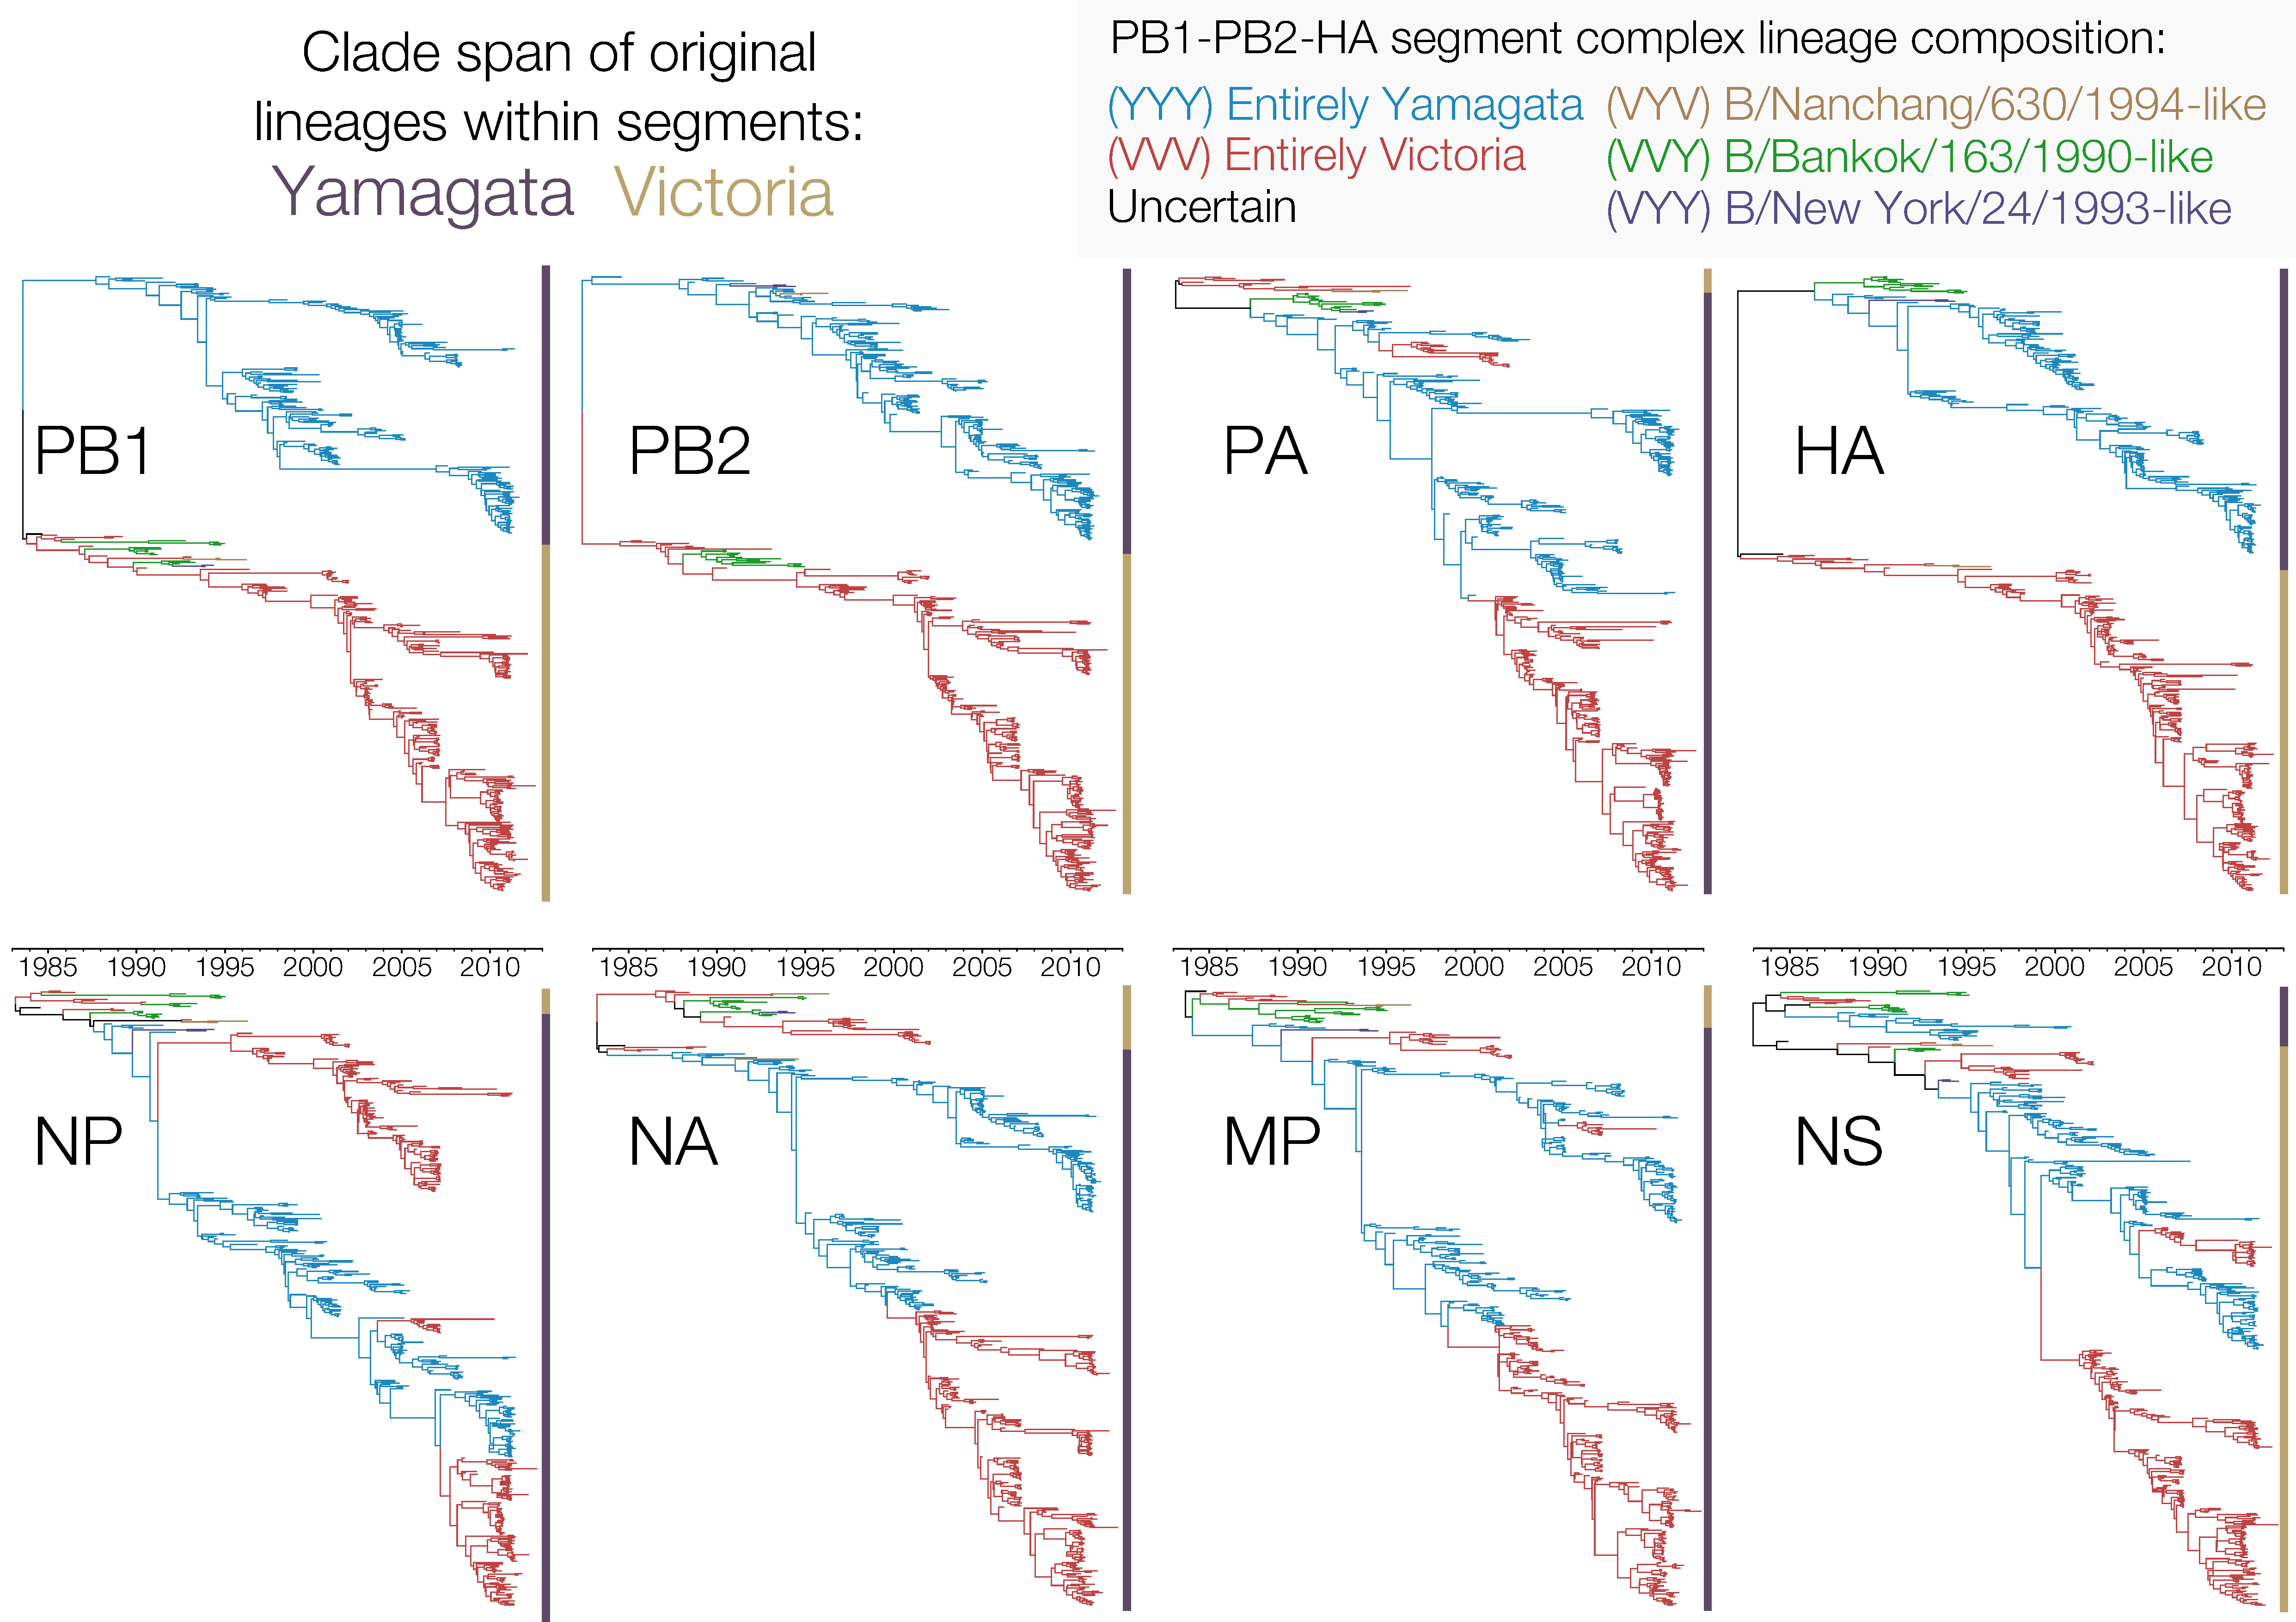
\includegraphics[width=0.95\textwidth]  {supp_figures/InfB_genomeGrid.pdf}
\caption{\textbf{MCC trees of 8 segments.}
Maximum clade credibility trees of all 8 genome segments of influenza B viruses isolated since 1980.
Trees are coloured based on inferred PB1-PB2-HA lineage.
Vertical bars indicate the original Victoria and Yamagata lineages within each segment.}
\label{genomeGrid}
\end{figure}

\section*{Linkage disequilibrium data}

\begin{figure}
\centering  
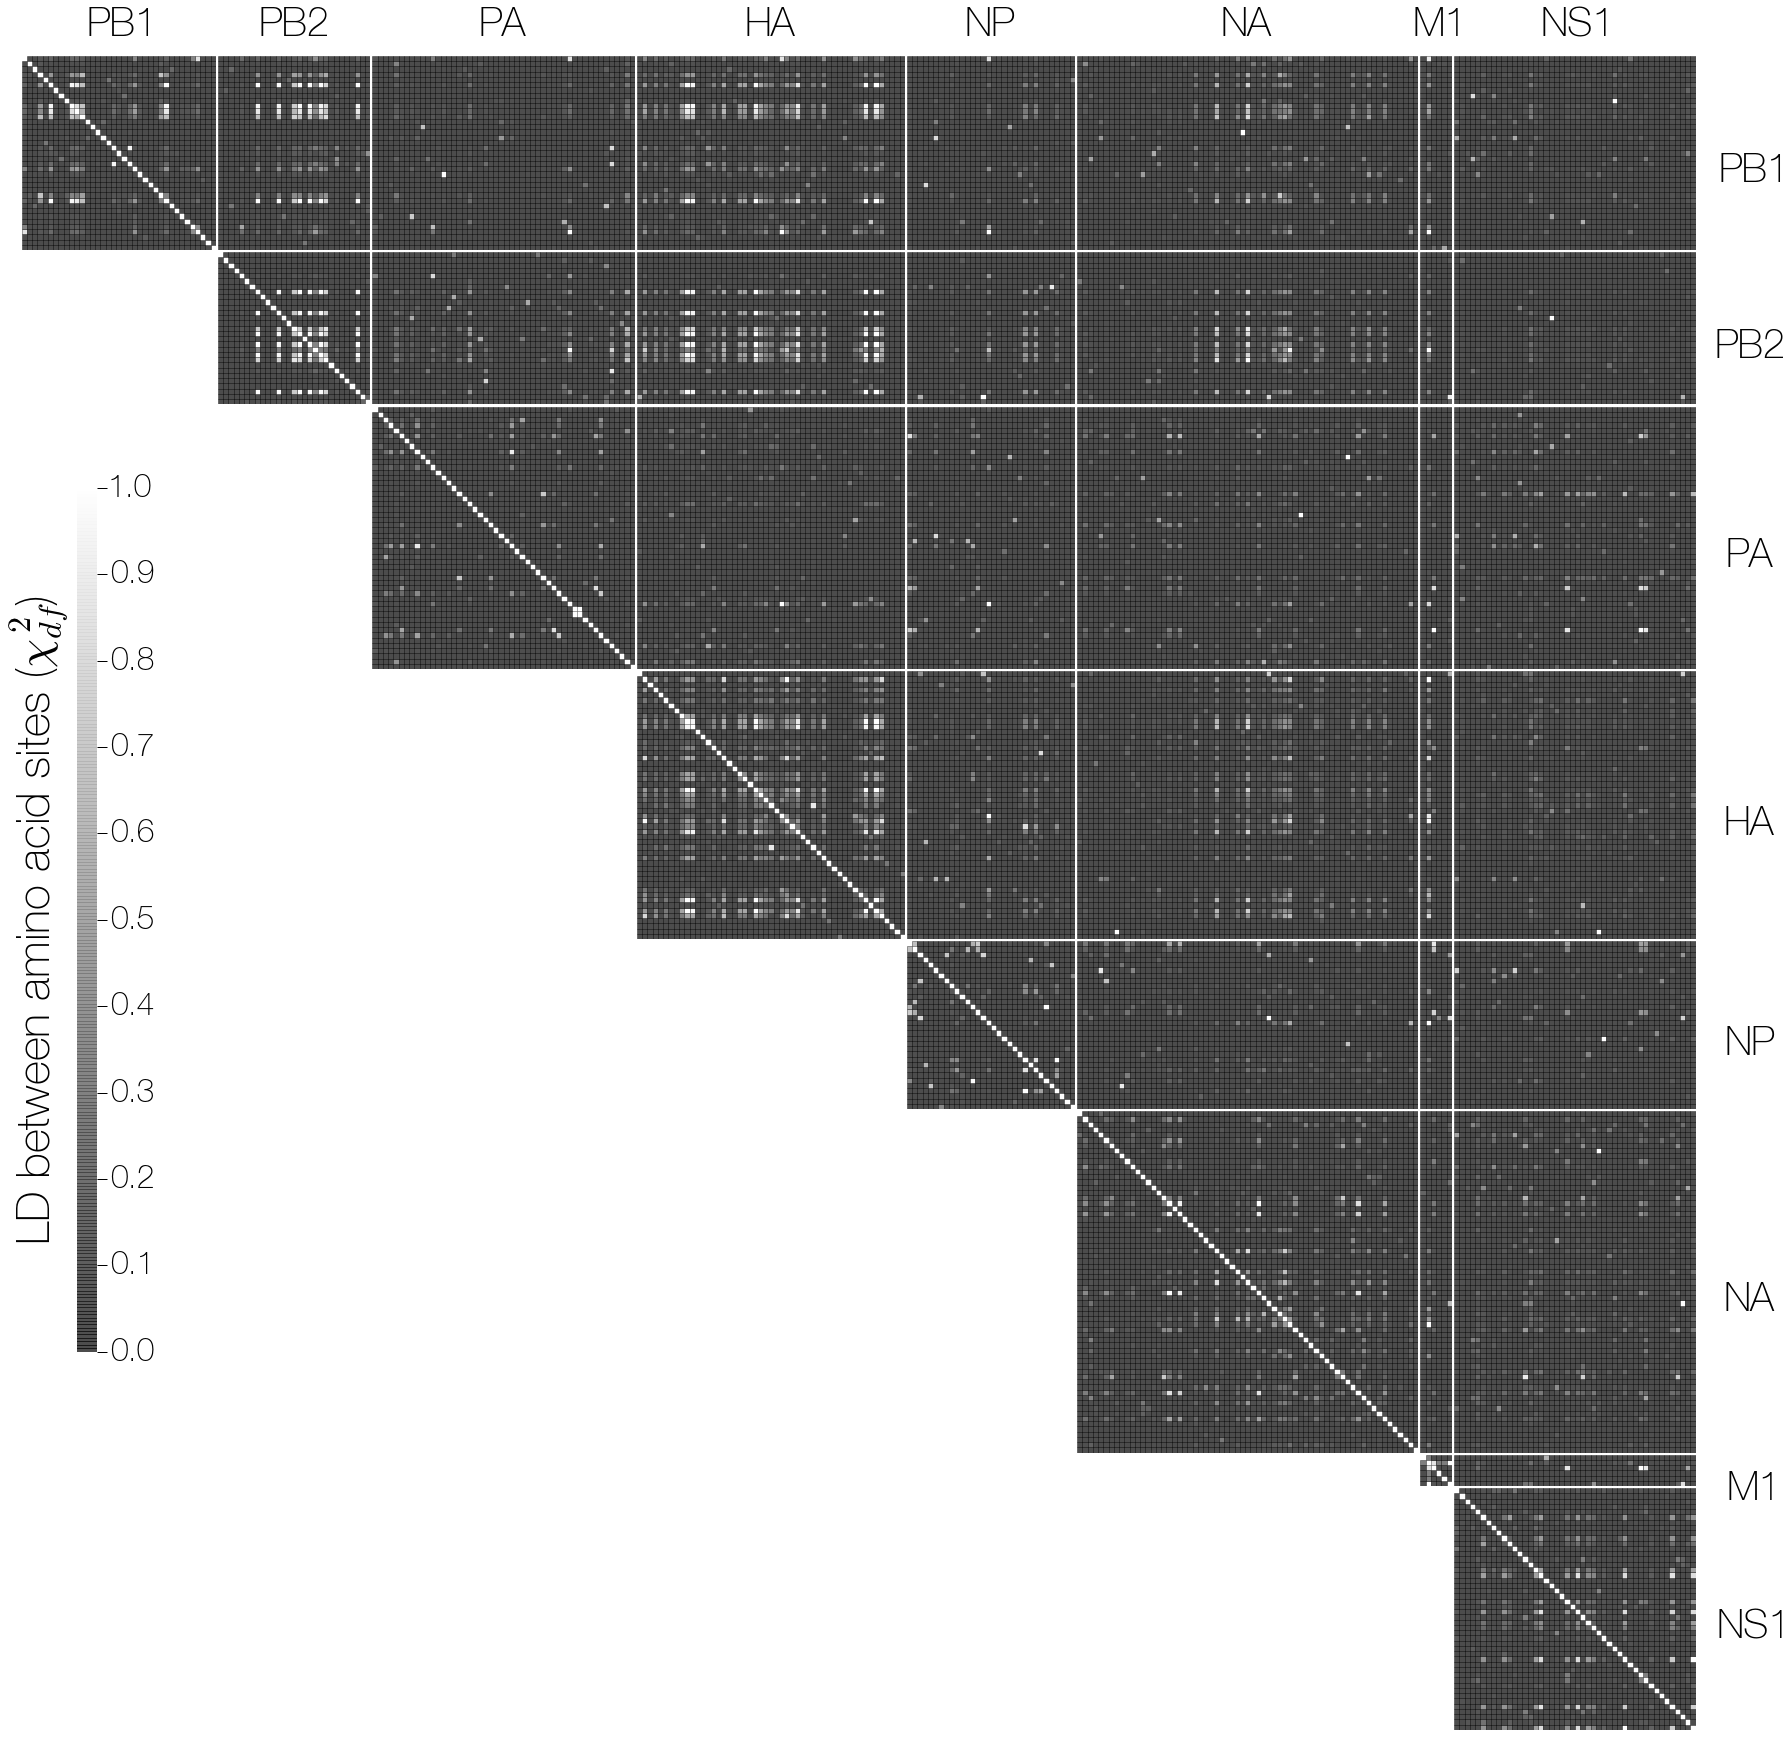
\includegraphics[width=0.95\textwidth]  {supp_figures/aaChi_Genome.png}
\caption{\textbf{Heatmap of genome-wide linkage disequilibrium ($\chi^{2}_{df}$) between polymorphic amino acid sites.}
Patterns of LD across the genome suggest a network of reciprocally linked amino acid sites on PB1, PB2, HA and to some extent NA proteins.
Proximity of sites on heatmaps might not correspond to proximity of sites within proteins.}
\label{ChiGenome}
\end{figure}

\begin{figure}
\centering  
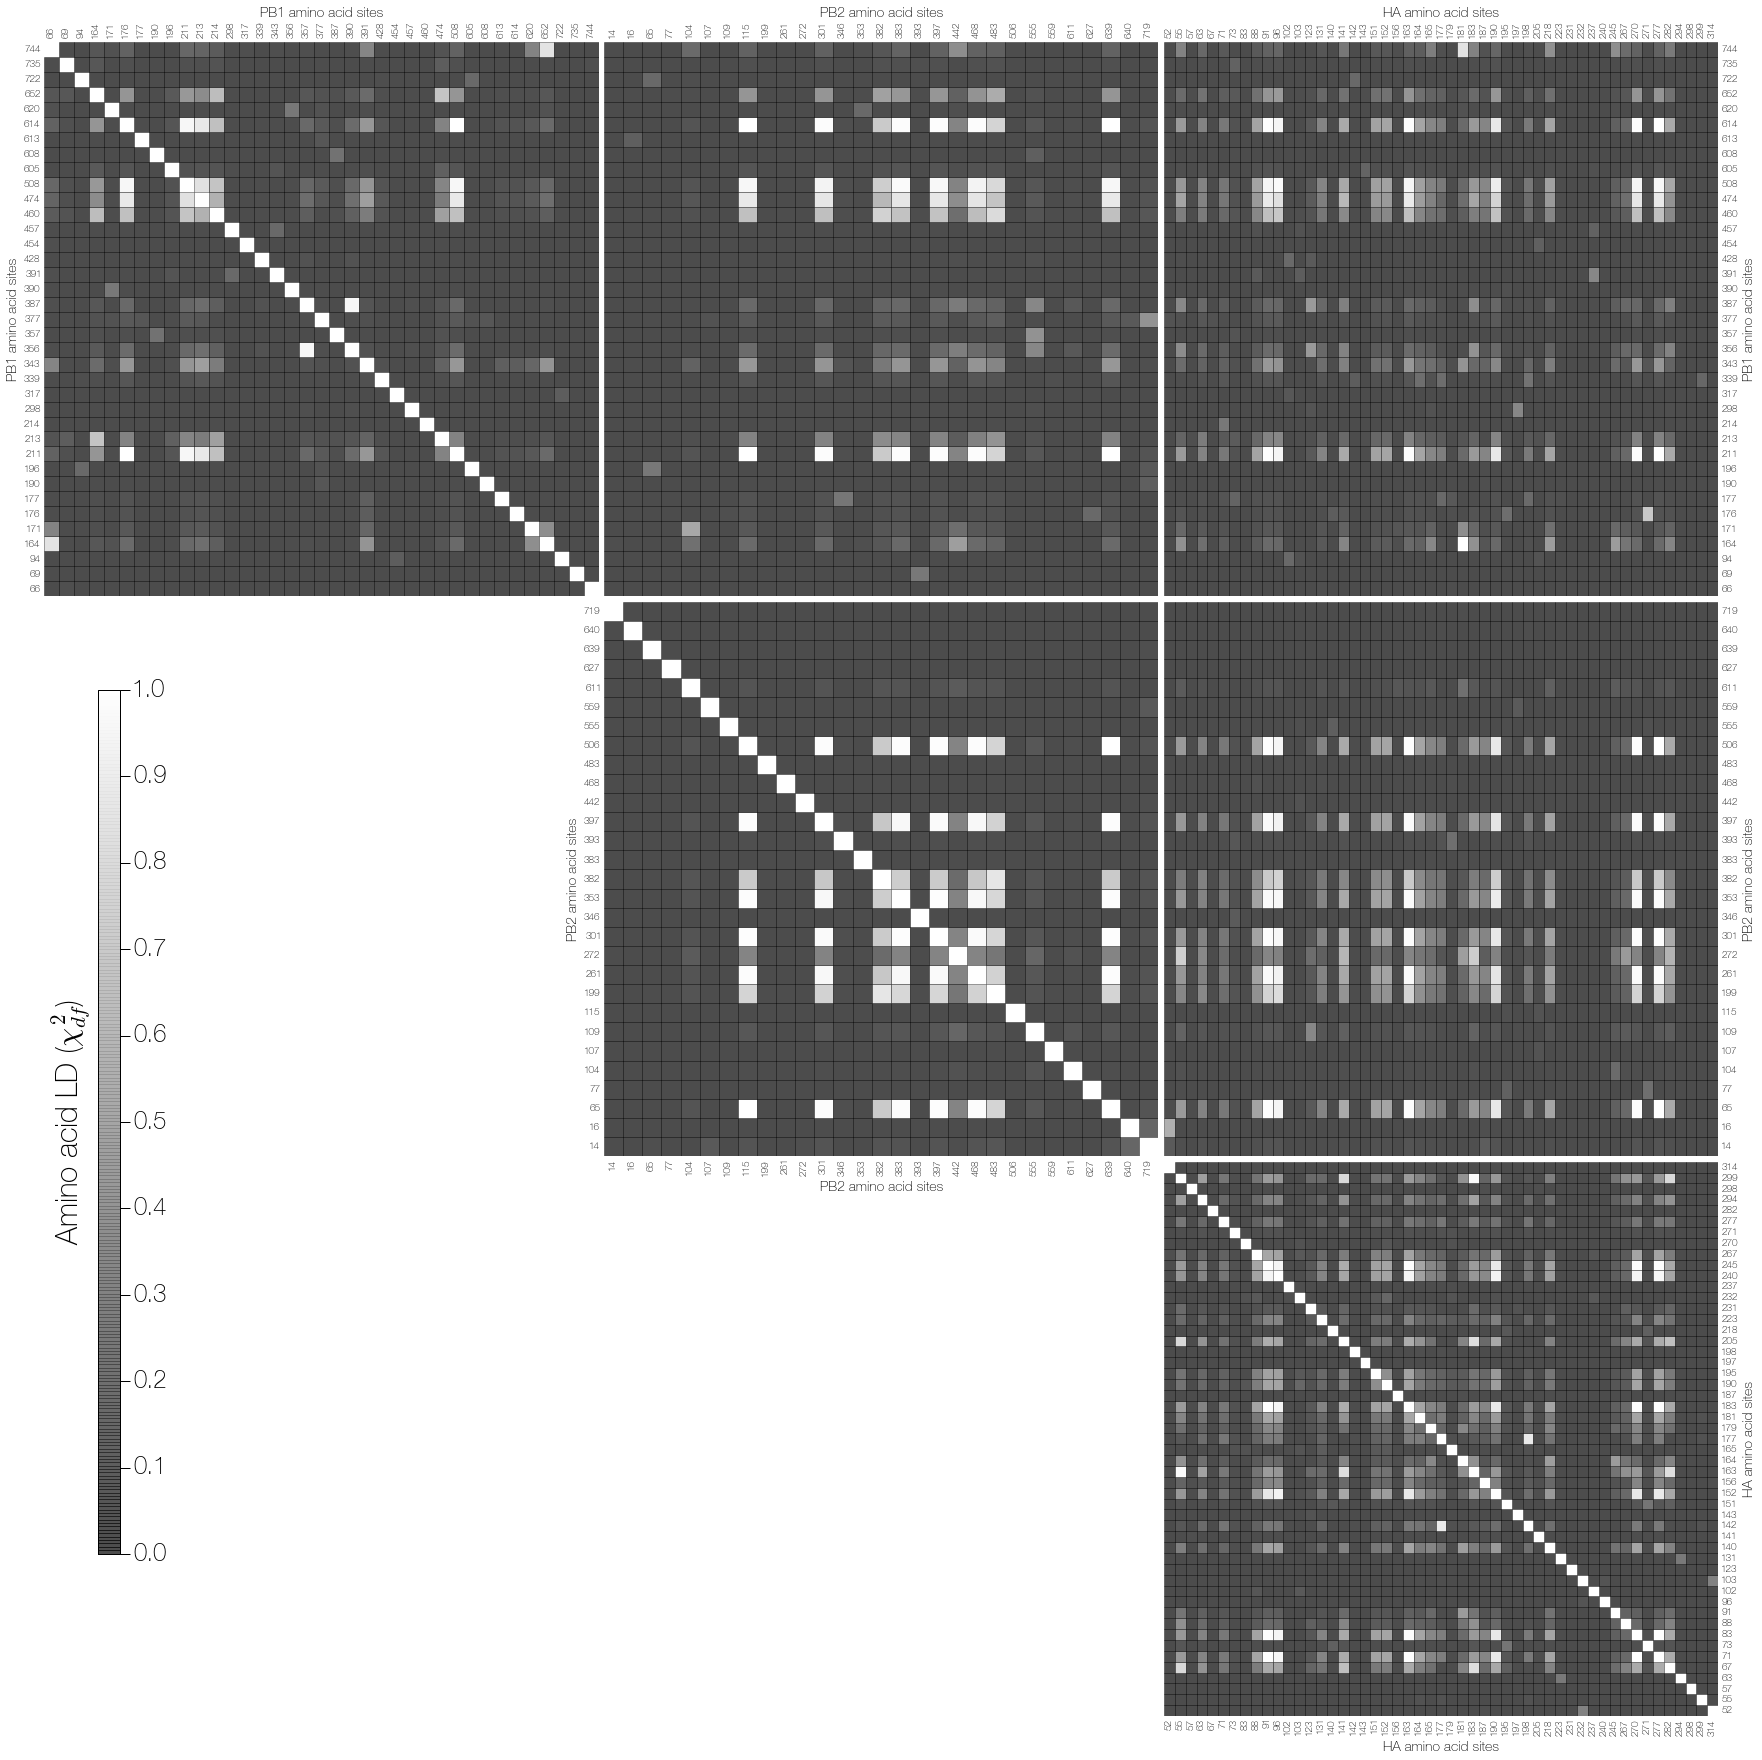
\includegraphics[width=0.85\textwidth]  {supp_figures/aaChi_PB1_PB2_HA.png}
\caption{\textbf{Heatmap of linkage disequilibrium ($\chi^{2}_{df}$) between amino acid sites on PB1, PB2 and HA proteins.}
Numbers next to each row and column correspond to amino acid site number within a given protein starting from methionine.}
\label{ChiCore}
\end{figure}

We have identified amino acid sites which exhibit a high degree of linkage disequilibrium between PB1, PB2 and HA segments.
Sites with high LD on PB1, PB2 and HA segments could be interpreted as either sites which have drifted apart due to lack of reassortment between the three segments or as sites which prevent the cooperation of the three proteins at the molecular level and thus prevent inter-lineage PB1-PB2-HA reassortants from having comparable fitness to viruses with `pure' lineage PB1-PB2-HA complexes.

None of the sites we have identified on PB1 and PB2 proteins fall within the previously described regions that form the contacts between the two polymerase subunits \cite{sugiyama2009}.

Sites 211, 213 and 214 on the PB1 protein are very close to each other and the stretch of sequence around these residues contains many positively charged amino acids (lysine and arginine).
Multiple nuclear localization signals (NLSs) are predicted to occur around this region and sites 211, 213 and 214 are either predicted to be near the end of a mono-partite NLS or the beginning of a bi-partite NLS.
Previous research \cite{nath1990} suggests that in the influenza A PB1 protein residue 211 (homologous to influenza B PB1 residue 211) is the last residue of a bi-partite NLS.
Almost all Yamagata lineage isolates possess arginine (R) residue at PB1 positions 211 and 214 and a serine (S) residue at position 213, whereas Victoria lineage isolates have lysine (K) at positions 211 and 214 and threonine (T) at position 213.
It remains to be seen whether these sites significantly affect the nuclear import efficiency of the PB1 protein of either lineage.
Though the PB1 protein is known to accumulate in the nucleus on its own, efficient import into the nucleus requires the presence of the PA protein \cite{fodor2004}.
Similarly, sites 382 and 397 on the PB2 protein are close to residues 377, 406 and 408 which are homologous to sites in influenza A that are responsible for mRNA cap-binding \cite{guilligay2008}.
Again, we cannot determine whether this finding is significant or not.

\section*{Tree-to-tree comparisons}

Figures \ref{SPRdistancesTrees} and \ref{SPRdistancesReplicates} are showing approximate SPR distances prior to the normalization procedure (see Methods).
Figure \ref{SPRdistancesTrees} shows that MP and NS trees show greater approximate SPR distances when compared to any other segment tree, which is consistent with the fact that only M1 and NS1 coding sequences, which are shorter than any other coding sequences, were used to infer the trees.
Figure \ref{SPRdistancesReplicates} confirms this by showing greater variability in tree topology (as greater approximate SPR distance) when MP and NS trees are compared against their replicates.
For all other segments approximate SPR distances between all pairs of trees prior to normalization suggests that most segment pairs have similar posterior distributions of approximate SPR distances.

\begin{figure}
\centering  
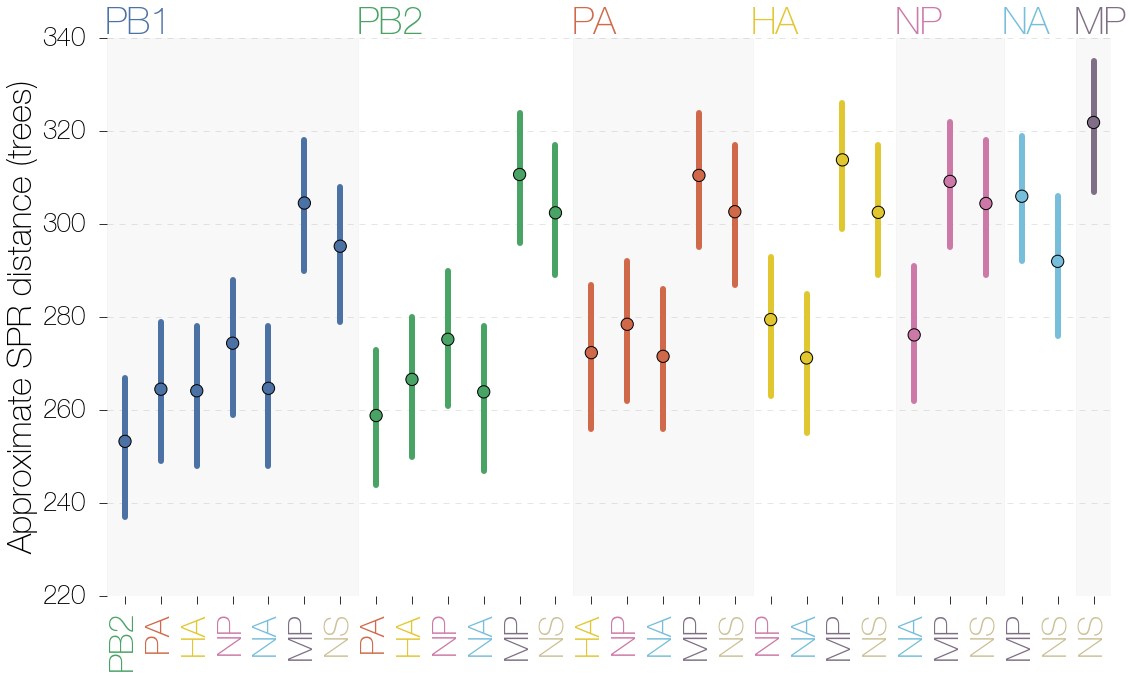
\includegraphics[width=0.65\textwidth]  {supp_figures/InfB_supp_aSPRdistances_trees.png}
\caption{\textbf{Approximate SPR distances between all pairs of trees of segments.}}
\label{SPRdistancesTrees}
\end{figure}

\begin{figure}
\centering  
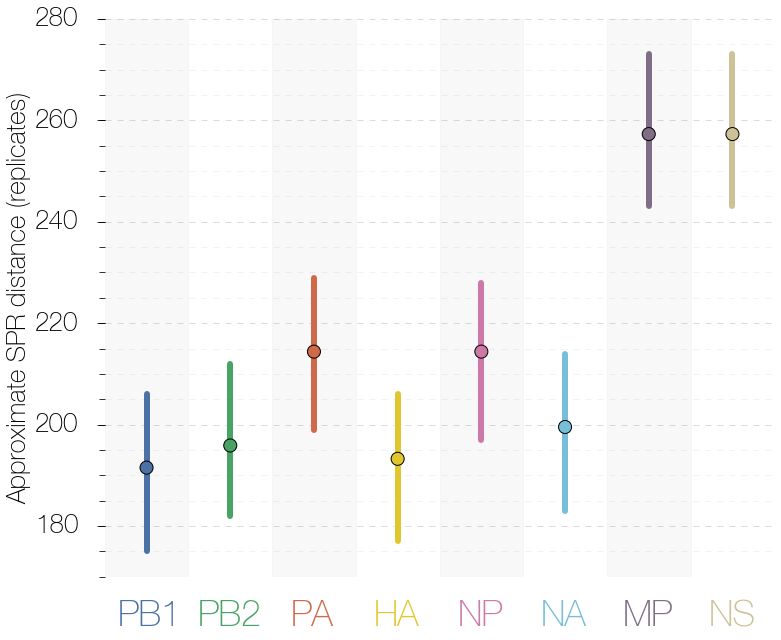
\includegraphics[width=0.65\textwidth]  {supp_figures/InfB_supp_aSPRdistances_replicates.png}
\caption{\textbf{Approximate SPR distances between replicate trees of each segment.}}
\label{SPRdistancesReplicates}
\end{figure}

Figures \ref{deltaTMRCAtrees} and \ref{deltaTMRCAreplicates} show $\Delta$TMRCA statistics for inter-segment and intra-segment, respectively, comparisons prior to normalization.
Figure \ref{deltaTMRCAtrees} shows that similarity in TMRCAs (as low $\Delta$TMRCA) between PB1, PB2 and HA segments is due to considerably smaller $\Delta$TMRCA statistic for the comparison between these segments.
It is also noteworthy that NA and MP comparisons have similarly low values for this statistic.
Figure \ref{deltaTMRCAreplicates} shows that TMRCAs are quite robust over the course of MCMC and node times do not, even in the most extreme cases, deviate from their replicates by more than 1 year.

\begin{figure}
\centering  
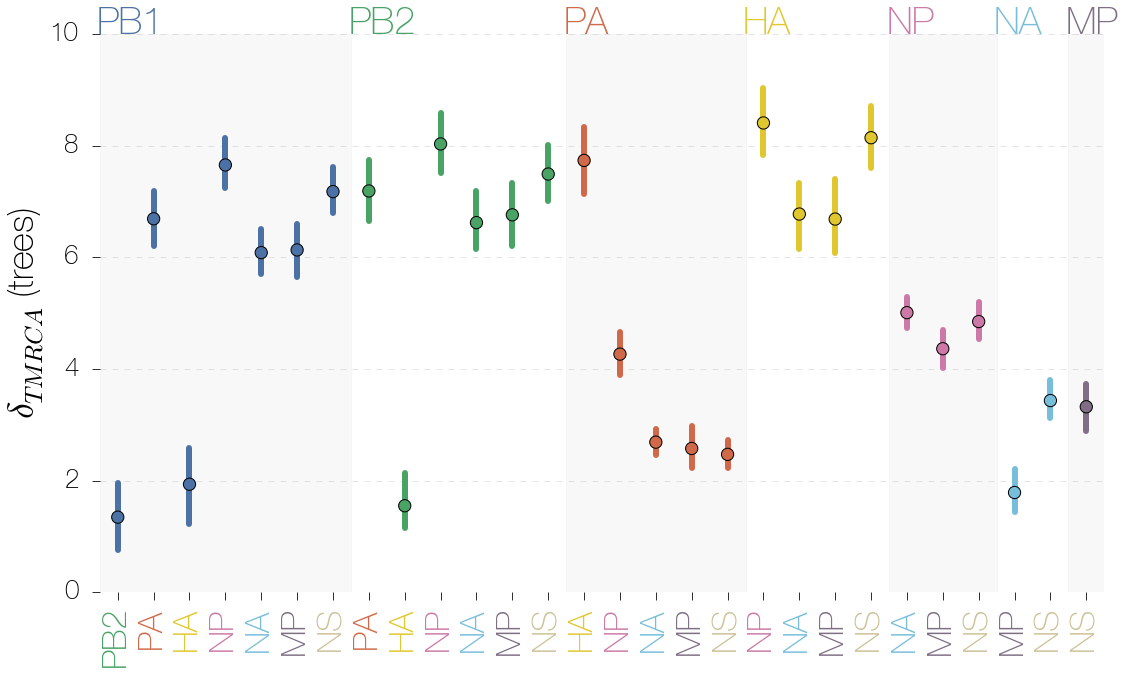
\includegraphics[width=0.65\textwidth]  {supp_figures/InfB_supp_deltaTMRCA_trees.png}
\caption{\textbf{Mean $\Delta$TMRCA between all pairs of trees of segments.}}
\label{deltaTMRCAtrees}
\end{figure}

\begin{figure}
\centering  
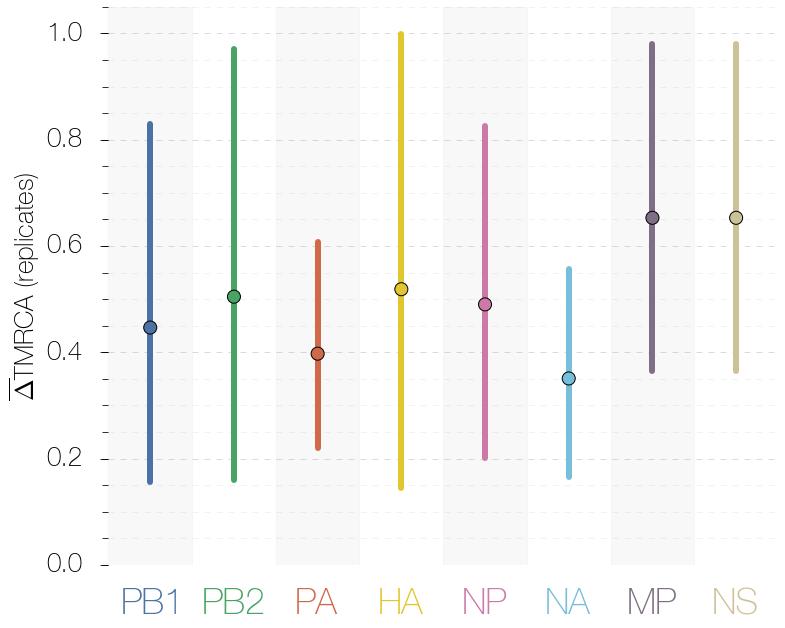
\includegraphics[width=0.65\textwidth]  {supp_figures/InfB_supp_deltaTMRCA_replicates.png}
\caption{\textbf{Mean $\Delta$TMRCA between replicate trees of each segment.}}
\label{deltaTMRCAreplicates}
\end{figure}

\begin{figure}
\centering  
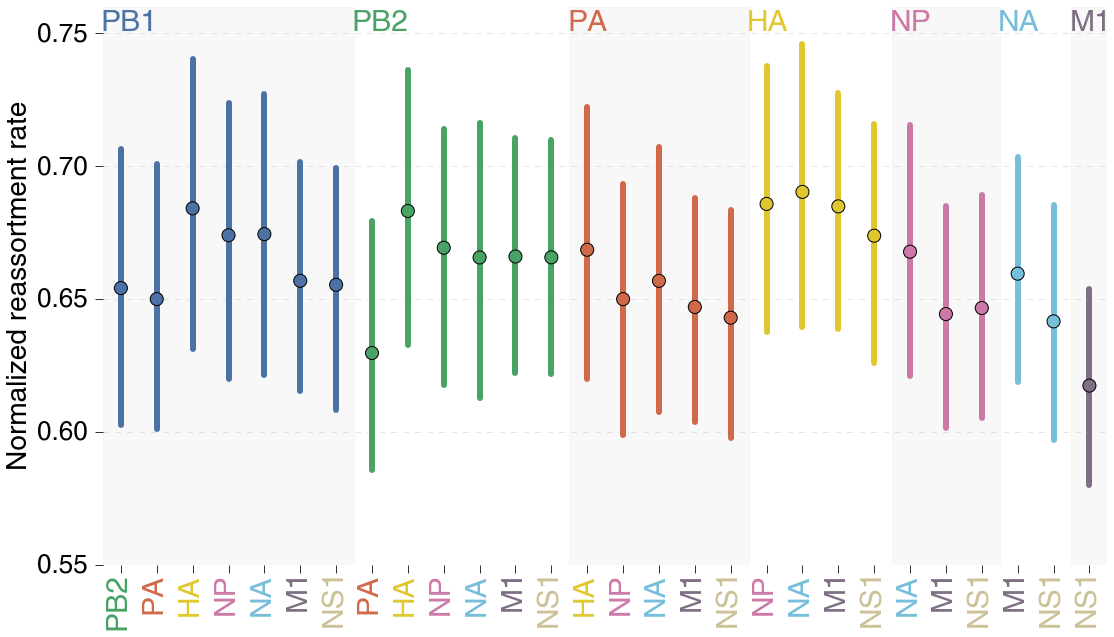
\includegraphics[width=0.65\textwidth]  {supp_figures/InfB_supp_normRErate.png}
\caption{\textbf{Normalized reassortment rate (approximate number of SPR moves per total time in both trees) between all pairs of trees of segments.}}
\label{NormSPR_RErate}
\end{figure}

We also tested the accuracy of approximate SPR distances using exact SPR distances calculated from PB1, PB2 and HA comparisons.
Figures \ref{SPR_PB1-PB2_difference}--\ref{SPR_PB2-HA_ratio} show that after normalization the approximate and exact SPR distance estimates are not significantly different.
There is also good correlation between the two SPR distances (Figures \ref{SPR_PB1-PB2_correlation}--\ref{SPR_PB2-HA_correlation}). 
Due to excessively long computation time of exact SPR distances very few PB2--HA comparisons were made.

\begin{figure}
\centering  
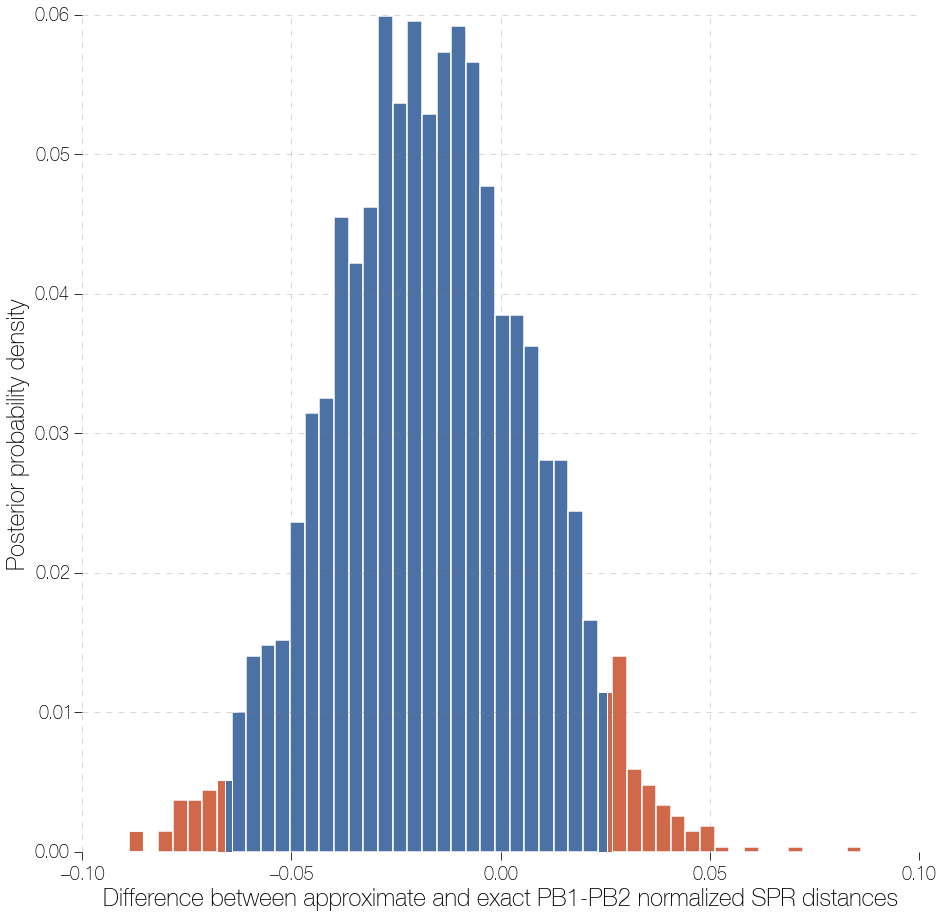
\includegraphics[width=0.65\textwidth]  {supp_figures/InfB_supp_NormPB1-PB2_hist.png}
\caption{\textbf{Distribution of differences between exact and approximate PB1-PB2 SPR distances after normalization.}}
\label{NormSPR_PB1-PB2_difference}
\end{figure}

\begin{figure}
\centering  
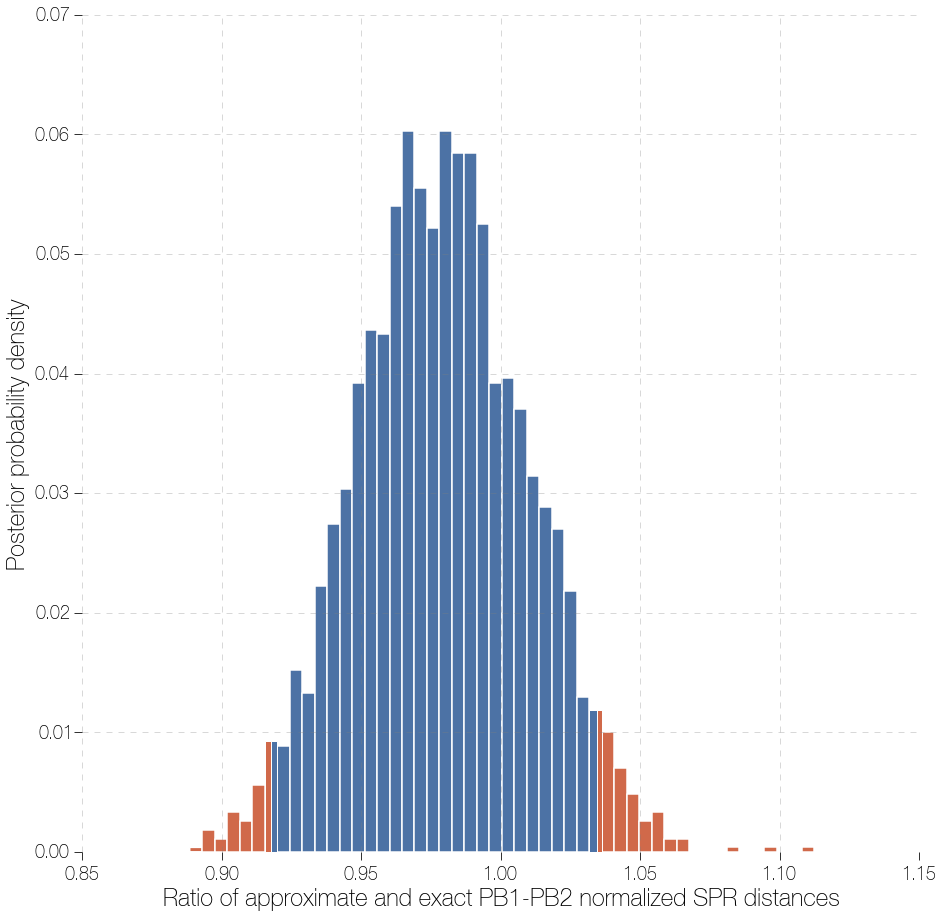
\includegraphics[width=0.65\textwidth]  {supp_figures/InfB_supp_NormPB1-PB2_hist2.png}
\caption{\textbf{Distribution of ratios between exact and approximate PB1-PB2 SPR distances after normalization.}}
\label{NormSPR_PB1-PB2_ratio}
\end{figure}

\begin{figure}
\centering  
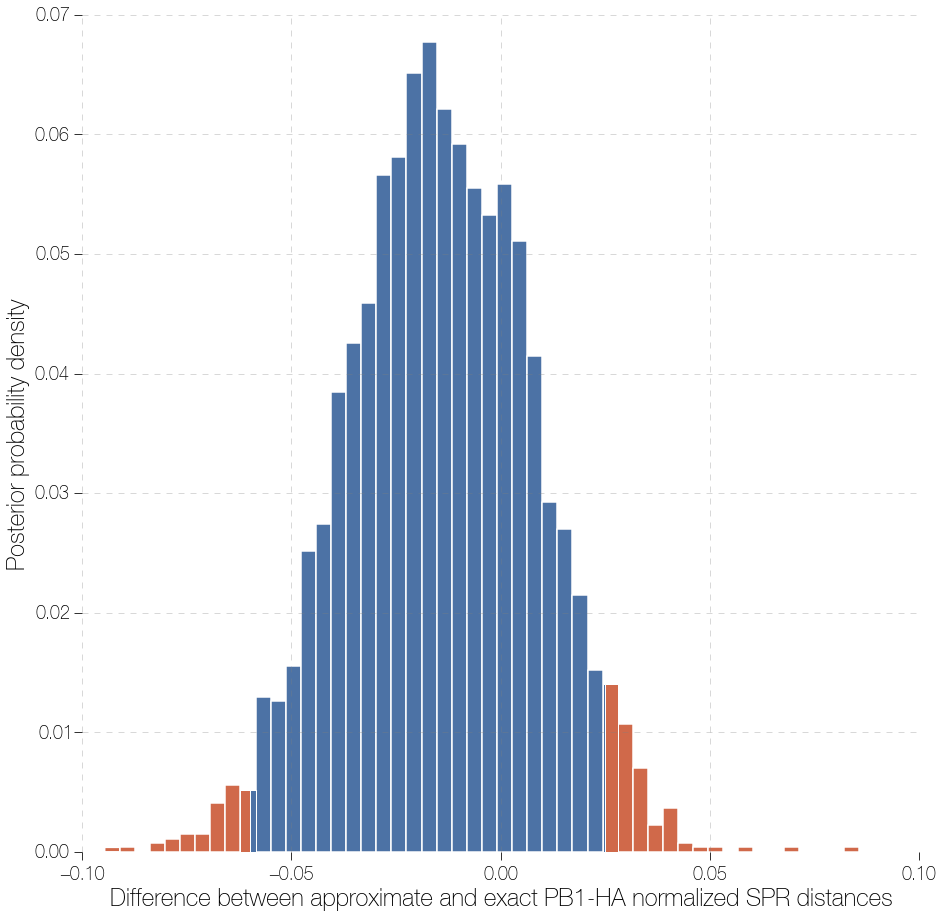
\includegraphics[width=0.65\textwidth]  {supp_figures/InfB_supp_NormPB1-HA_hist.png}
\caption{\textbf{Distribution of differences between exact and approximate PB1-HA SPR distances after normalization.}}
\label{NormSPR_PB1-HA_difference}
\end{figure}

\begin{figure}
\centering  
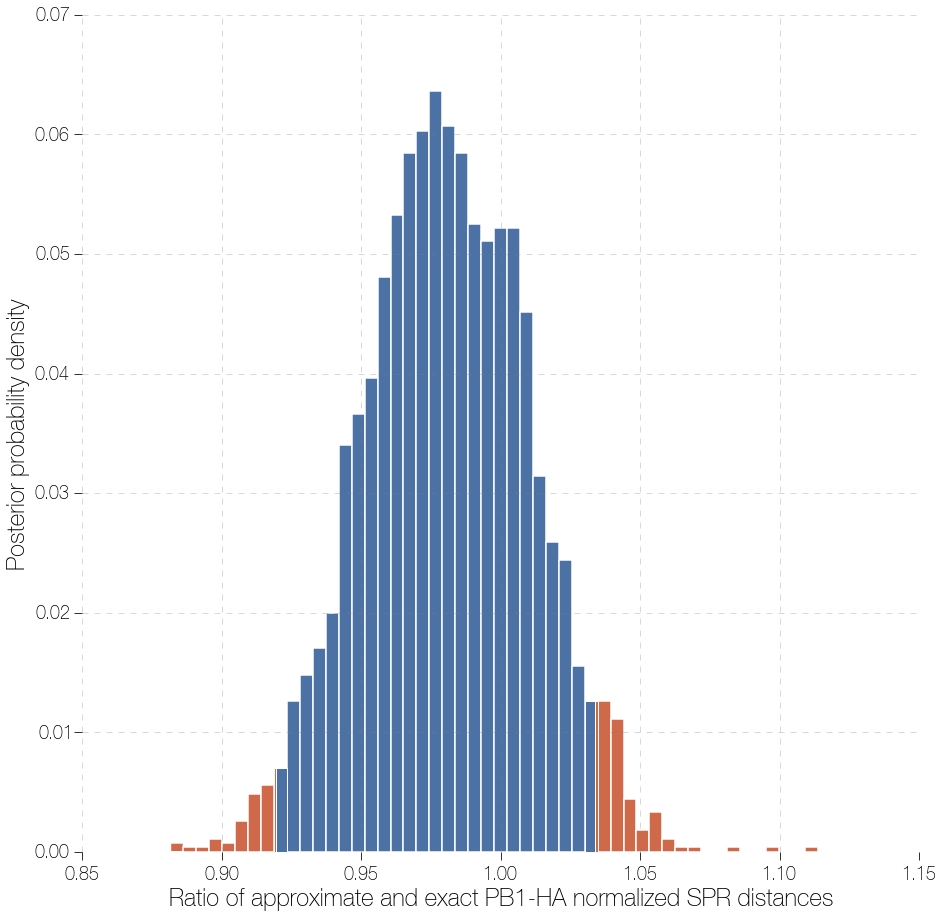
\includegraphics[width=0.65\textwidth]  {supp_figures/InfB_supp_NormPB1-HA_hist2.png}
\caption{\textbf{Distribution of ratios between exact and approximate PB1-HA SPR distances after normalization.}}
\label{NormSPR_PB1-HA_ratio}
\end{figure}

\begin{figure}
\centering  
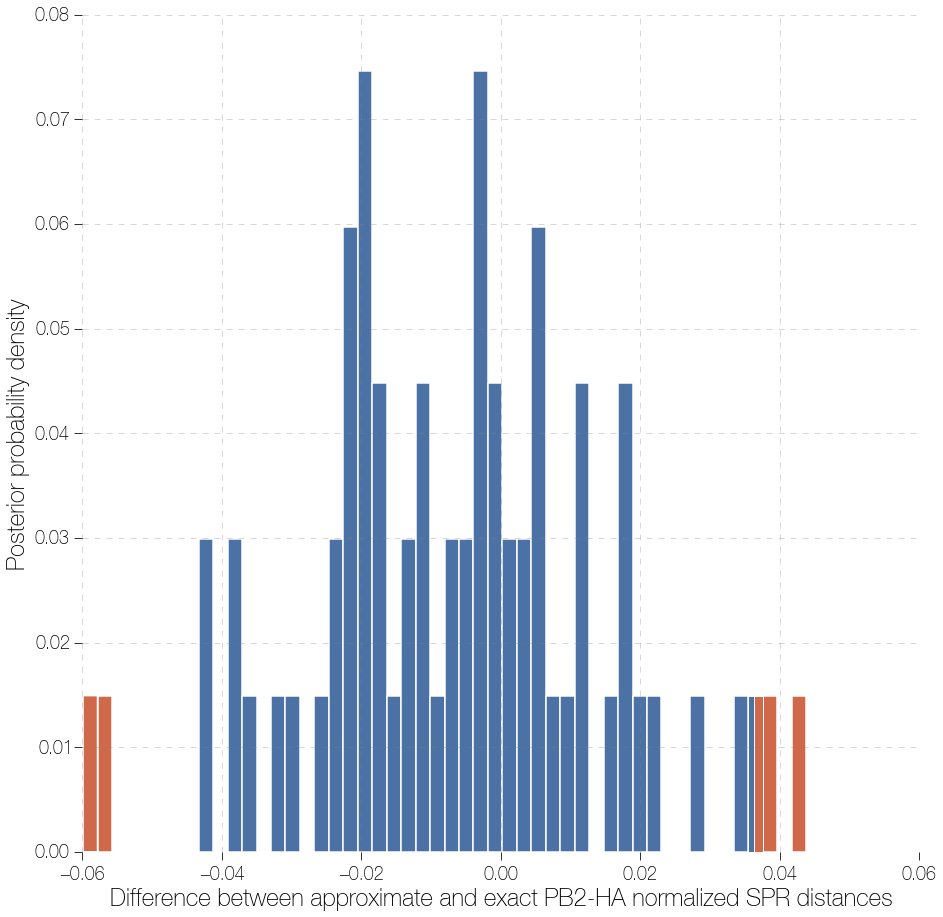
\includegraphics[width=0.65\textwidth]  {supp_figures/InfB_supp_NormPB2-HA_hist.png}
\caption{\textbf{Distribution of differences between exact and approximate PB2-HA SPR distances after normalization.}}
\label{NormSPR_PB2-HA_difference}
\end{figure}

\begin{figure}
\centering  
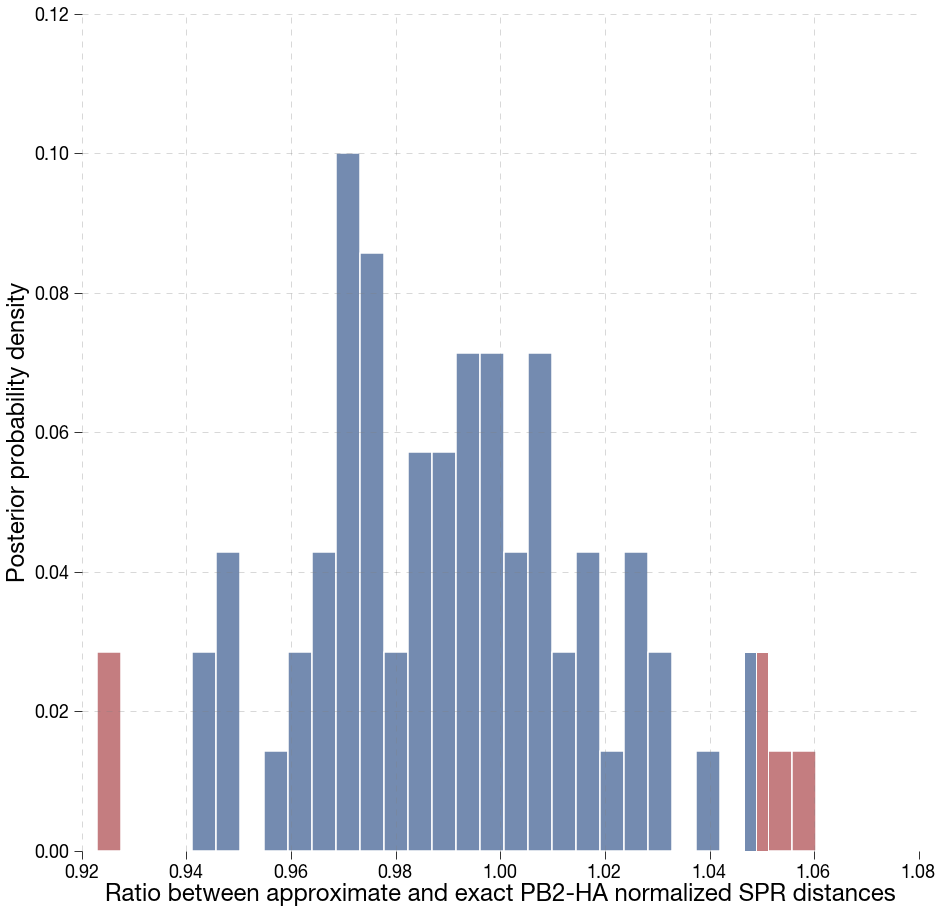
\includegraphics[width=0.65\textwidth]  {supp_figures/InfB_supp_PB2-HA_hist2.png}
\caption{\textbf{Distribution of ratios between exact and approximate PB2-HA SPR distances after normalization.}}
\label{NormSPR_PB2-HA_ratio}
\end{figure}

\begin{figure}
\centering  
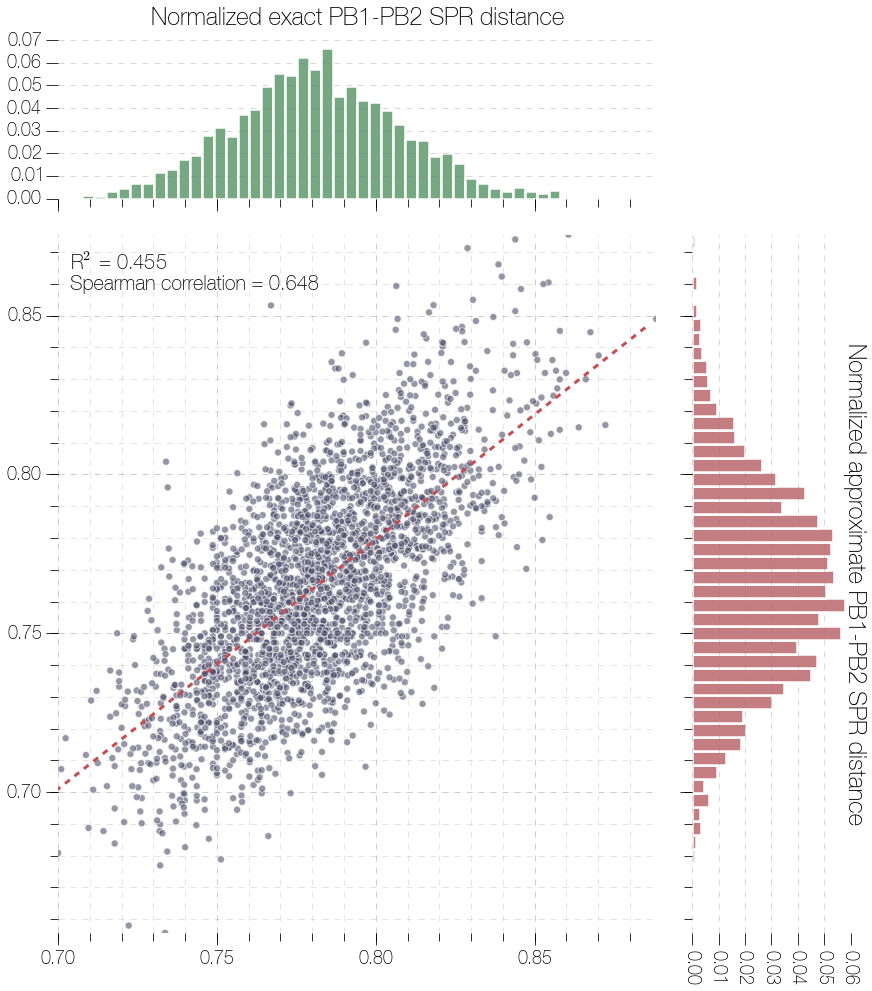
\includegraphics[width=0.5\textwidth]  {supp_figures/InfB_supp_NormPB1-PB2_corr.png}
\caption{\textbf{Correlation between exact and approximate PB1-PB2 SPR distances after normalization.}}
\label{NormSPR_PB1-PB2_correlation}
\end{figure}

\begin{figure}
\centering  
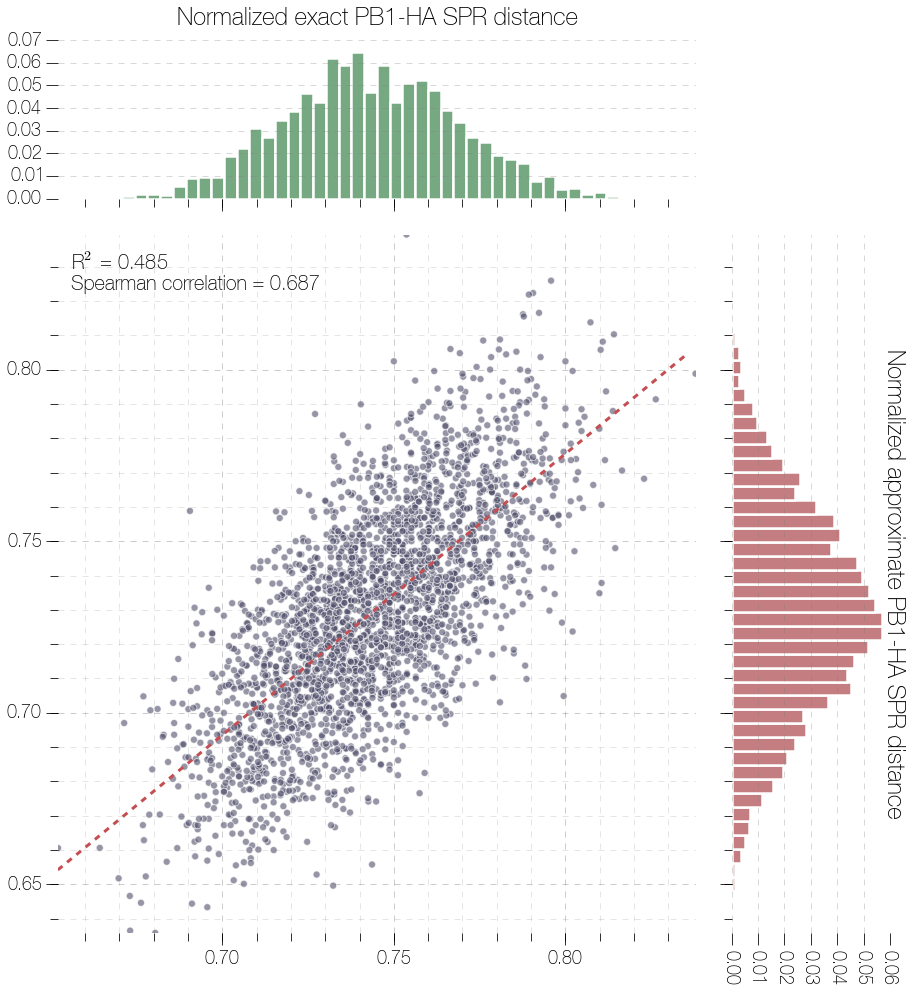
\includegraphics[width=0.5\textwidth]  {supp_figures/InfB_supp_NormPB1-HA_corr.png}
\caption{\textbf{Correlation between exact and approximate PB1-HA SPR distances after normalization.}}
\label{NormSPR_PB1-HA_correlation}
\end{figure}

\begin{figure}
\centering  
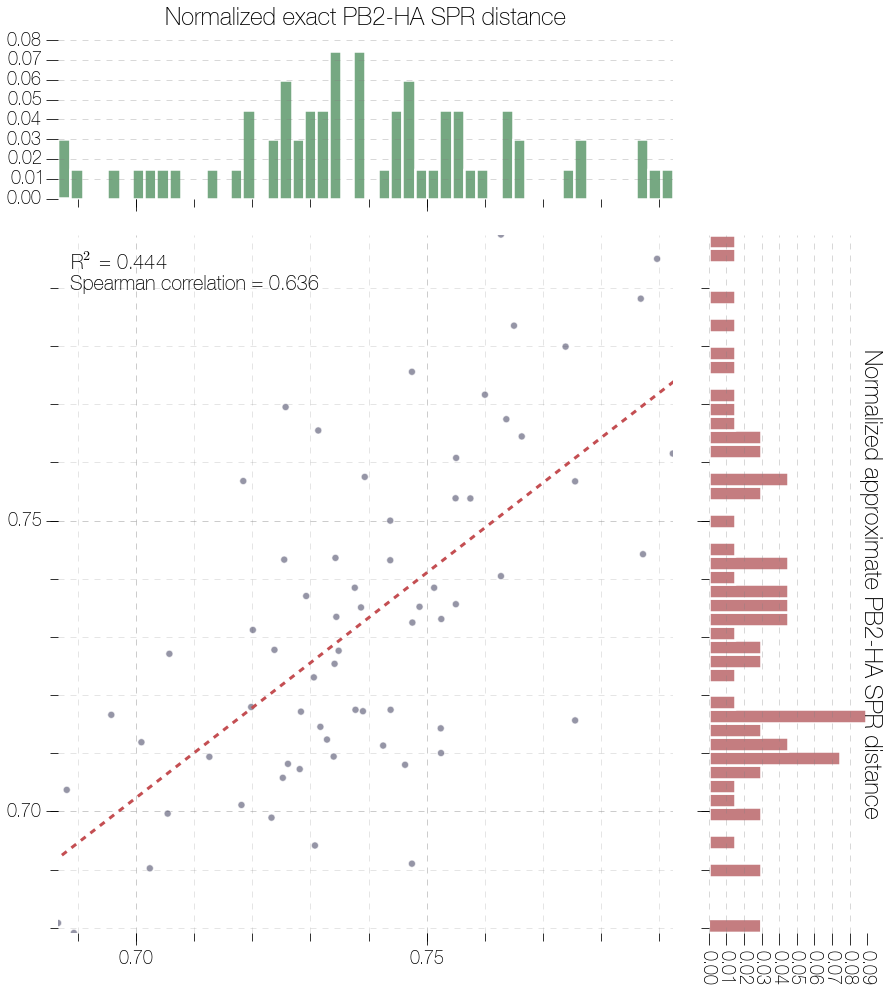
\includegraphics[width=0.5\textwidth]  {supp_figures/InfB_supp_NormPB2-HA_corr.png}
\caption{\textbf{Correlation between exact and approximate PB2-HA SPR distances after normalization.}}
\label{NormSPR_PB2-HA_correlation}
\end{figure}

\clearpage

Figures \ref{SPR_PB1-PB2_difference}--\ref{SPR_PB2-HA_ratio} focus on differences between exact and approximate SPR distances and show that prior to normalization approximate SPR distances are overestimates of exact SPR distances.
Figures \ref{SPR_PB1-PB2_correlation}--\ref{SPR_PB2-HA_correlation} show that there is a similar degree of correspondence between approximate and exact SPR distances to when approximate and exact SPR distances are normalized (Figures \ref{NormSPR_PB1-PB2_correlation}--\ref{NormSPR_PB2-HA_correlation}) using the procedure described in Methods.

\begin{figure}
\centering  
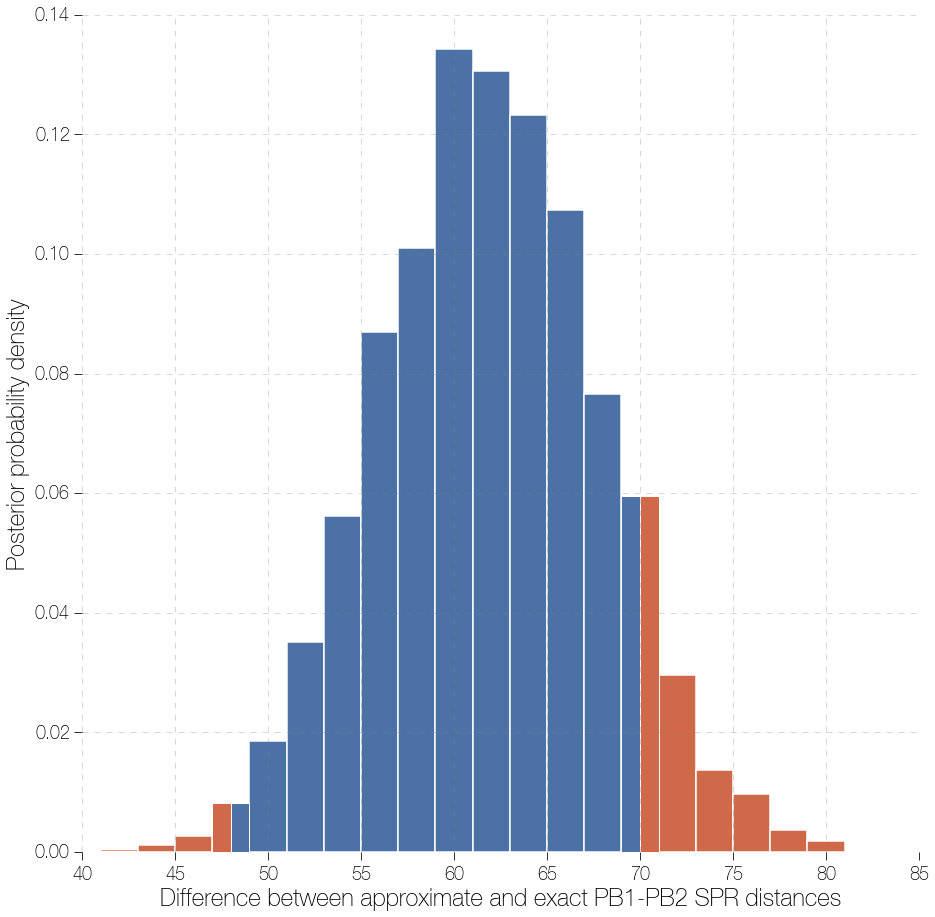
\includegraphics[width=0.65\textwidth]  {supp_figures/InfB_supp_PB1-PB2_hist.png}
\caption{\textbf{Distribution of differences between exact and approximate PB1-PB2 SPR distances.}}
\label{SPR_PB1-PB2_difference}
\end{figure}

\begin{figure}
\centering  
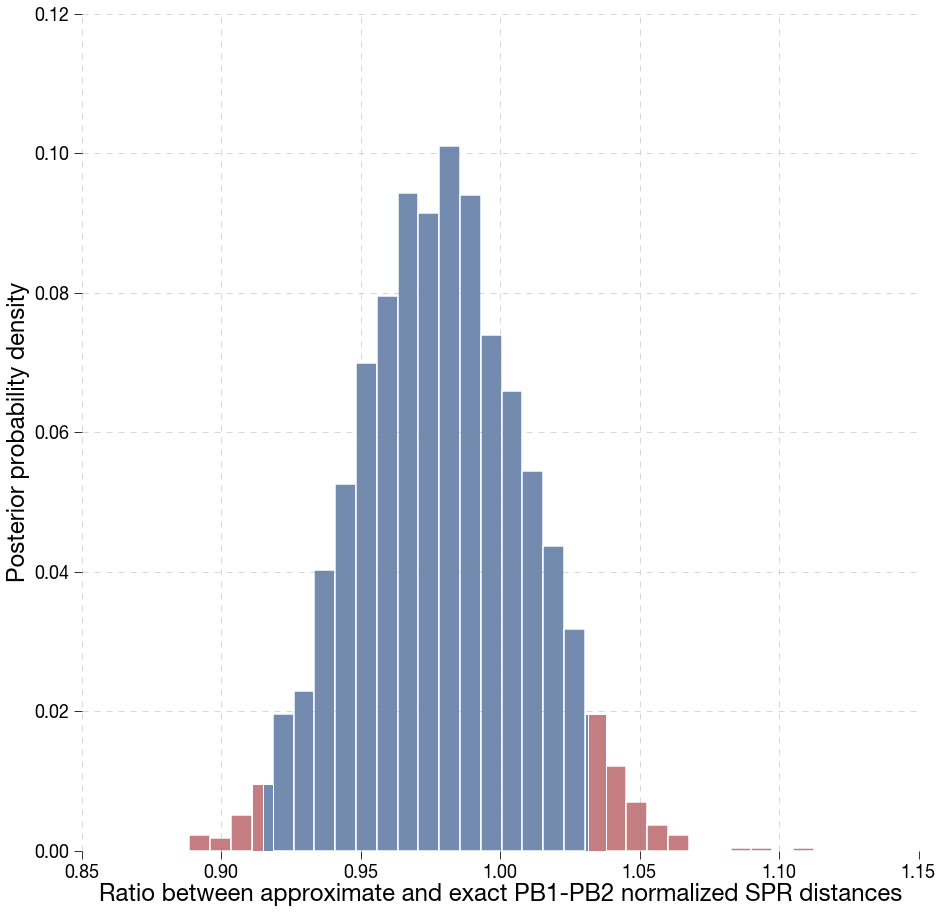
\includegraphics[width=0.65\textwidth]  {supp_figures/InfB_supp_PB1-PB2_hist2.png}
\caption{\textbf{Distribution of ratios between exact and approximate PB1-PB2 SPR distances.}}
\label{SPR_PB1-PB2_ratio}
\end{figure}

\begin{figure}
\centering  
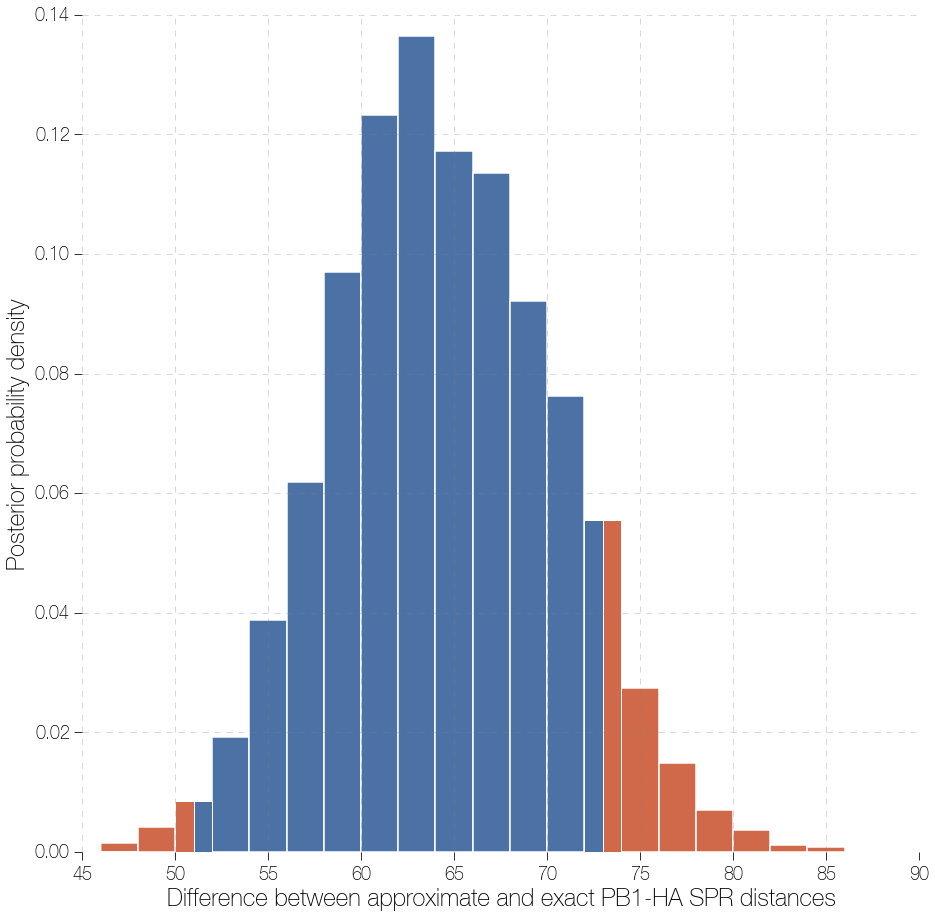
\includegraphics[width=0.65\textwidth]  {supp_figures/InfB_supp_PB1-HA_hist.png}
\caption{\textbf{Distribution of differences between exact and approximate PB1-HA SPR distances.}}
\label{SPR_PB1-HA_difference}
\end{figure}

\begin{figure}
\centering  
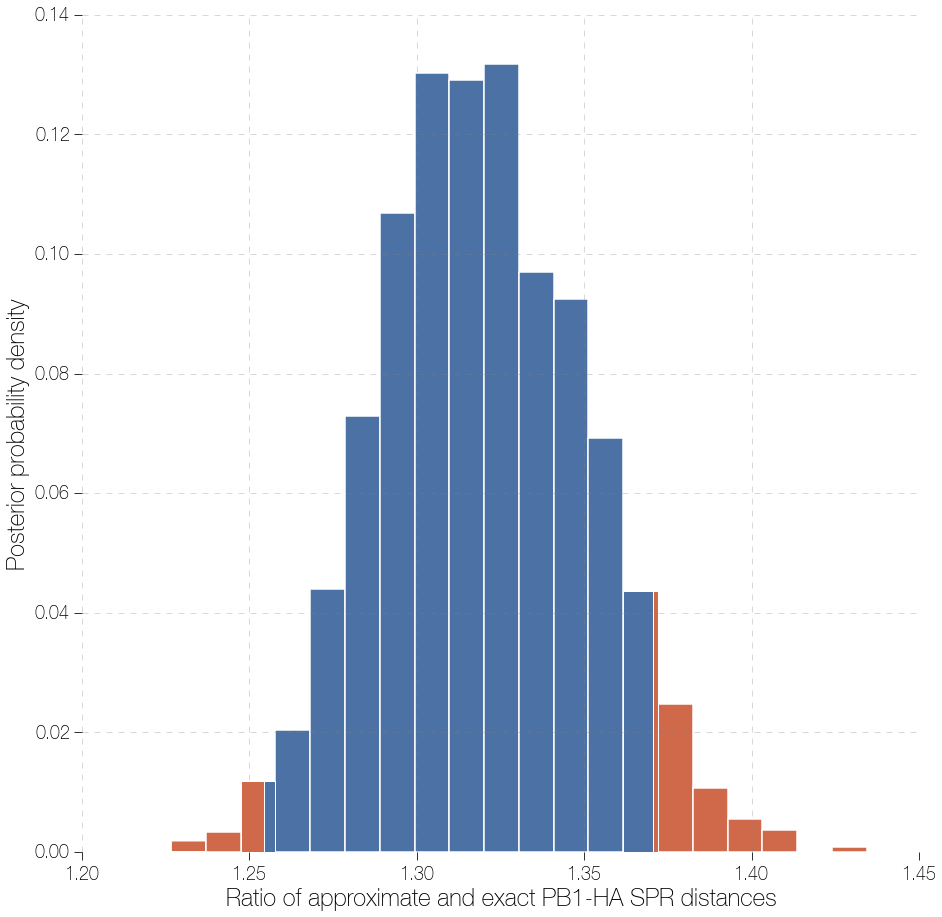
\includegraphics[width=0.65\textwidth]  {supp_figures/InfB_supp_PB1-HA_hist2.png}
\caption{\textbf{Distribution of ratios between exact and approximate PB1-HA SPR distances.}}
\label{SPR_PB1-HA_ratio}
\end{figure}

\begin{figure}
\centering  
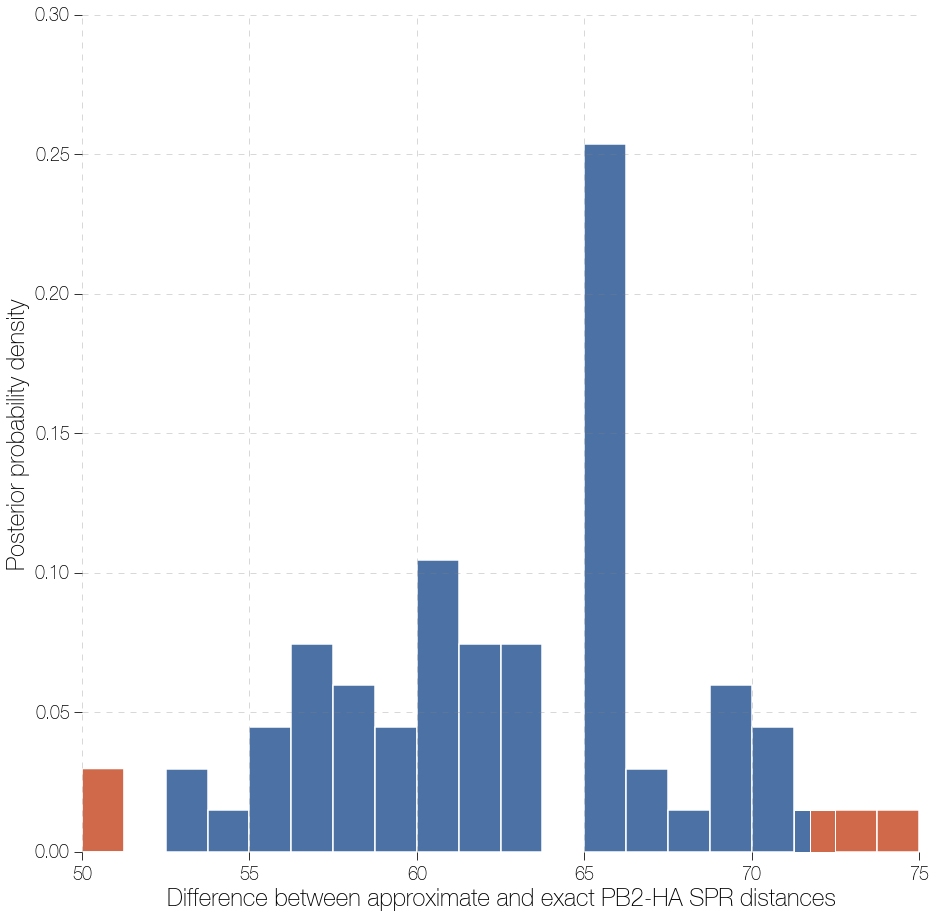
\includegraphics[width=0.65\textwidth]  {supp_figures/InfB_supp_PB2-HA_hist.png}
\caption{\textbf{Distribution of differences between exact and approximate PB2-HA SPR distances.}}
\label{SPR_PB2-HA_difference}
\end{figure}

\begin{figure}
\centering  
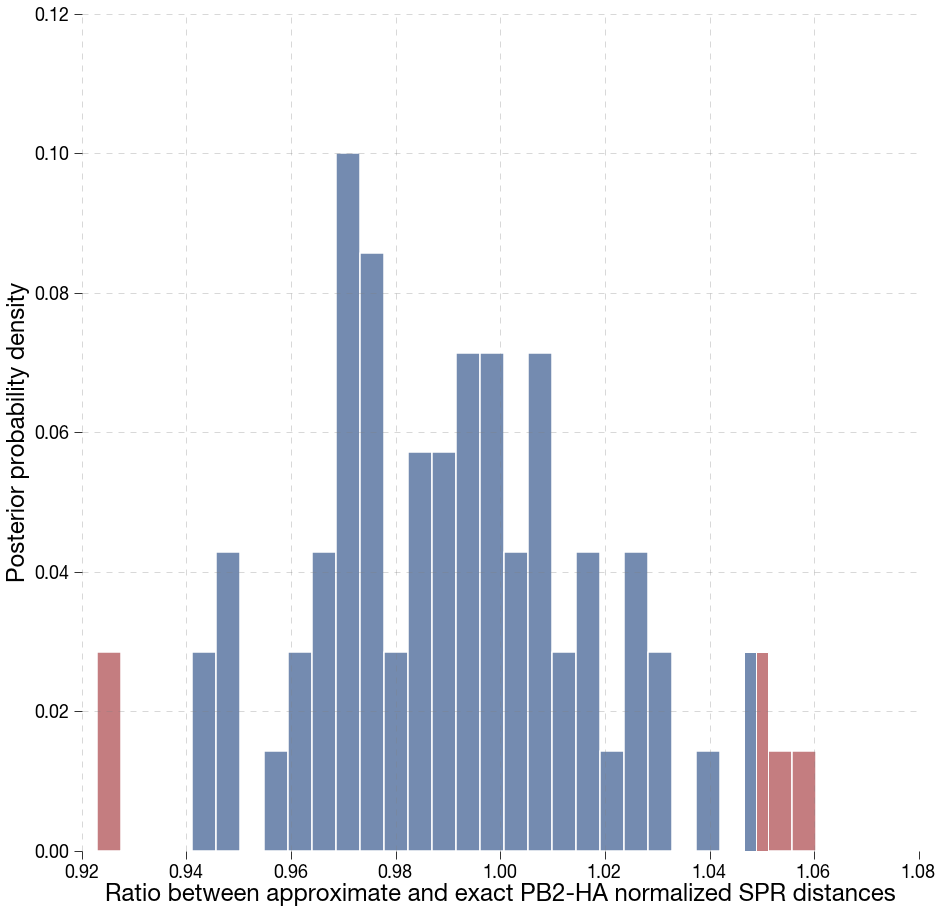
\includegraphics[width=0.65\textwidth]  {supp_figures/InfB_supp_PB2-HA_hist2.png}
\caption{\textbf{Distribution of ratios between exact and approximate PB2-HA SPR distances.}}
\label{SPR_PB2-HA_ratio}
\end{figure}

\begin{figure}
\centering  
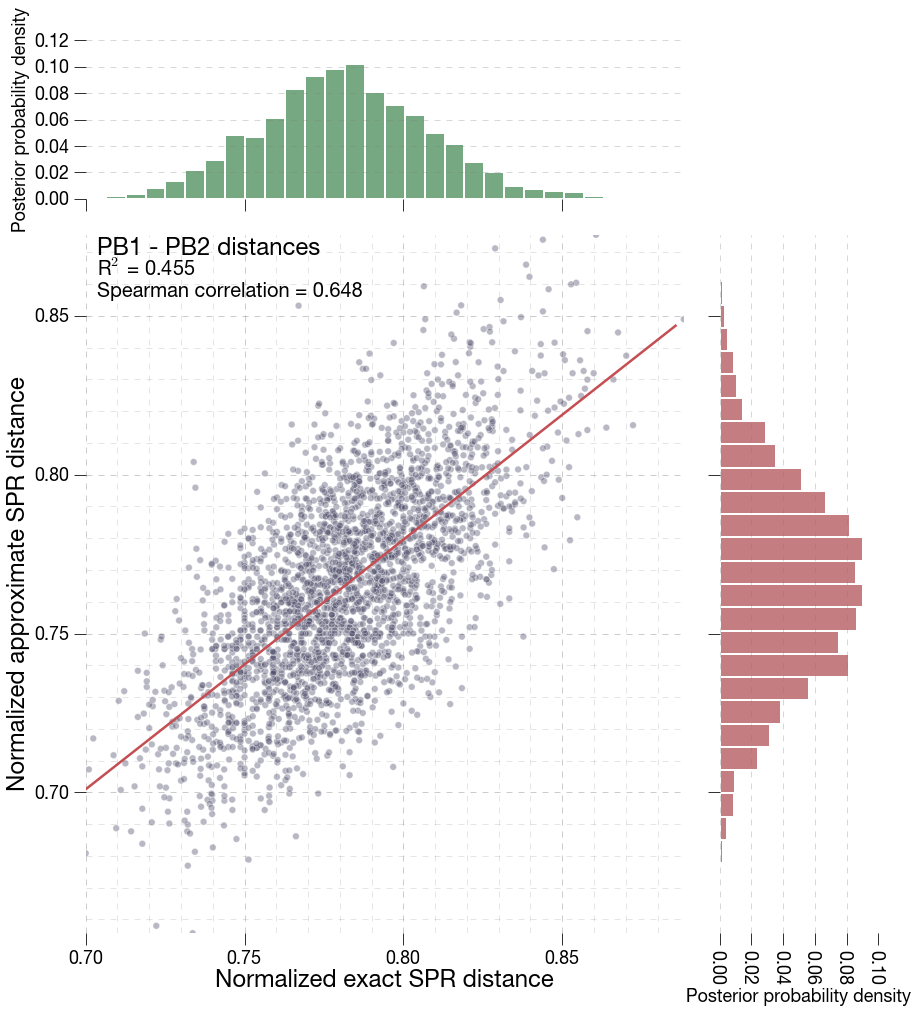
\includegraphics[width=0.4\textwidth]  {supp_figures/InfB_supp_PB1-PB2_corr.png}
\caption{\textbf{Correlation between exact and approximate PB1-PB2 SPR distances.}}
\label{SPR_PB1-PB2_correlation}
\end{figure}

\begin{figure}
\centering  
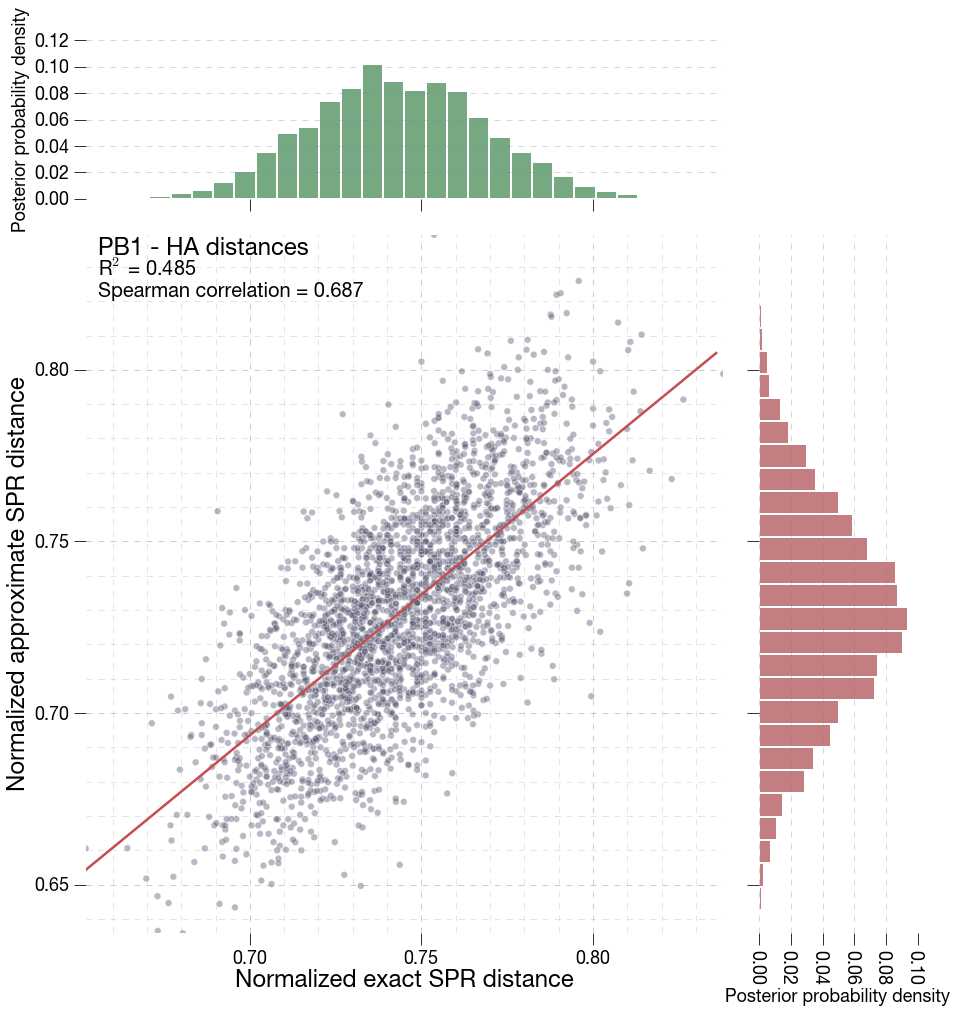
\includegraphics[width=0.4\textwidth]  {supp_figures/InfB_supp_PB1-HA_corr.png}
\caption{\textbf{Correlation between exact and approximate PB1-HA SPR distances.}}
\label{SPR_PB1-HA_correlation}
\end{figure}

\begin{figure}
\centering  
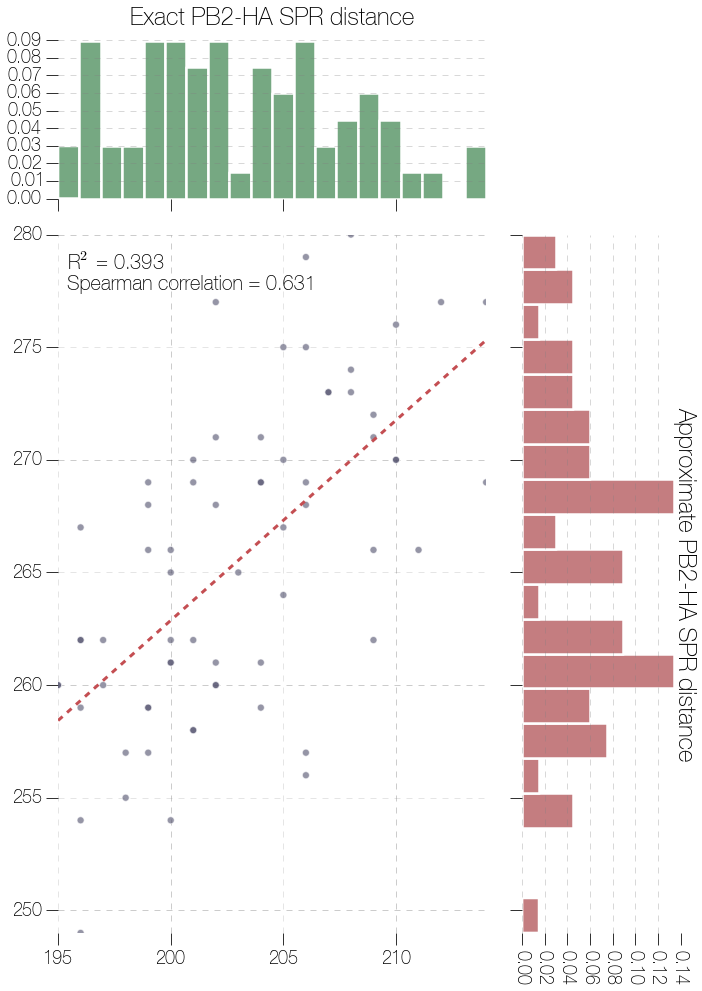
\includegraphics[width=0.4\textwidth]  {supp_figures/InfB_supp_PB2-HA_corr.png}
\caption{\textbf{Correlation between exact and approximate PB2-HA SPR distances.}}
\label{SPR_PB2-HA_correlation}
\end{figure}

\clearpage
\section*{Multidimensional scaling}
Figures \ref{MDSaaLD} and \ref{MDSntLD} visualize the relationships between segments based on mean amino acid and nucleotide site linkage disequilibrium estimates, respectively.
PB1, PB2 and HA segments appear to be by far the most similar segments, as indicated by their proximity in the MDS embedding.
Figures \ref{MDSaaCorr} and \ref{MDSntCorr} compare the observed mean LD values between segments. 
Based on mean amino acid site LD (Figure \ref{MDSaaCorr}) only PB1, PB2 and HA segments show considerable clustering, all other segments being equidistant from each other in the MDS embedding.
MDS distance versus mean nucleotide site LD scatter plot, on the other hand, shows a continuum of relationships between segments, which is probably caused by more variability at the nucleotide level than the amino acid level.
This difference in variability would build up linkage disequilibrium between nucleotide sites and would reduce it via convergent substitutions over relatively short periods of time.

\begin{figure}
\centering  
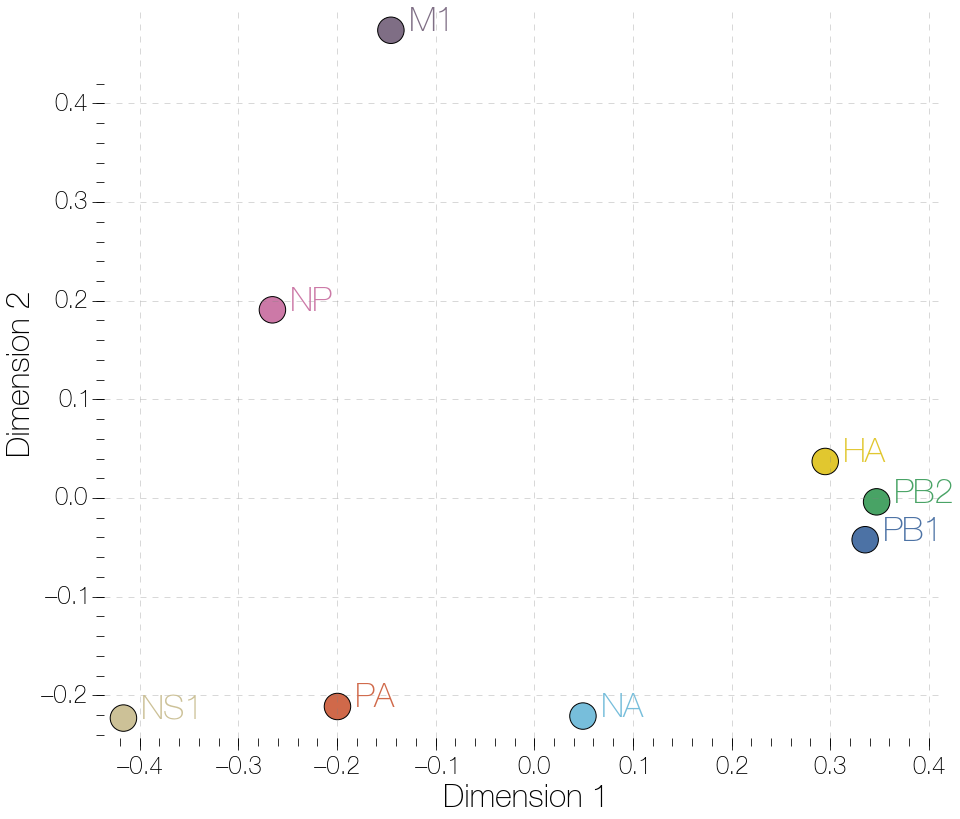
\includegraphics[width=0.65\textwidth]  {supp_figures/InfB_8x8_aaLD_MDS.png}
\caption{\textbf{2-dimensional MDS embedding of influenza B virus segments based on mean amino acid linkage disequilibrium ($\chi\_{df}^{2}$).}}
\label{MDSaaLD}
\end{figure}

\begin{figure}
\centering  
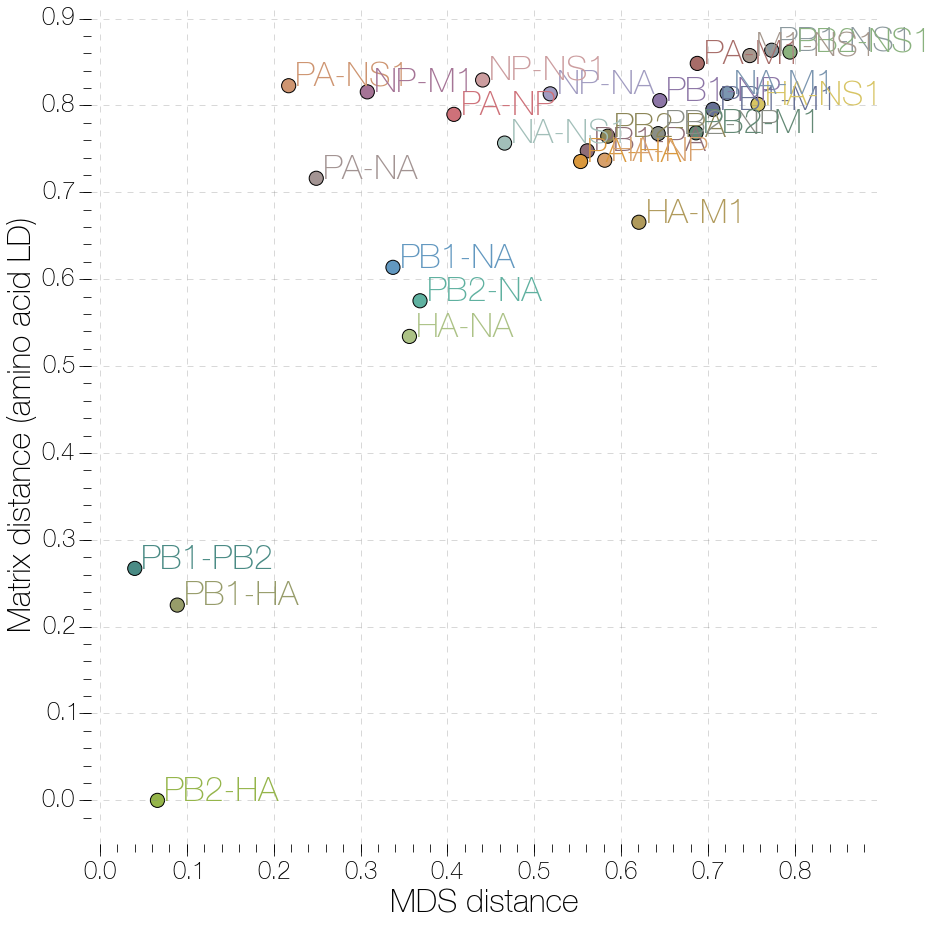
\includegraphics[width=0.65\textwidth]  {supp_figures/InfB_aaLD_MatrixMDScorr.png}
\caption{\textbf{Correlation between mean amino acid site linkage disequilibrium and MDS embedding distance for all pairs of segments.}}
\label{MDSaaCorr}
\end{figure}

\begin{figure}
\centering  
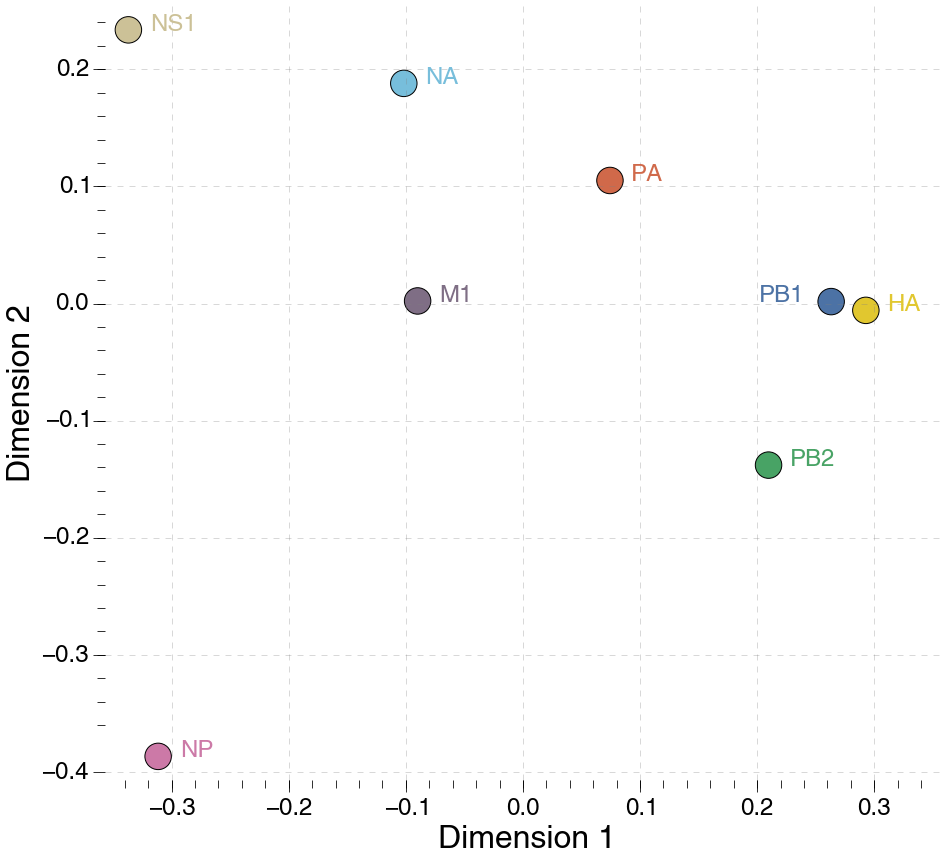
\includegraphics[width=0.65\textwidth]  {supp_figures/InfB_8x8_ntLD_MDS.png}
\caption{\textbf{2-dimensional MDS embedding of influenza B virus segments based on mean nucleotide linkage disequilibrium ($\chi\_{df}^{2}$).}}
\label{MDSntLD}
\end{figure}

\begin{figure}
\centering  
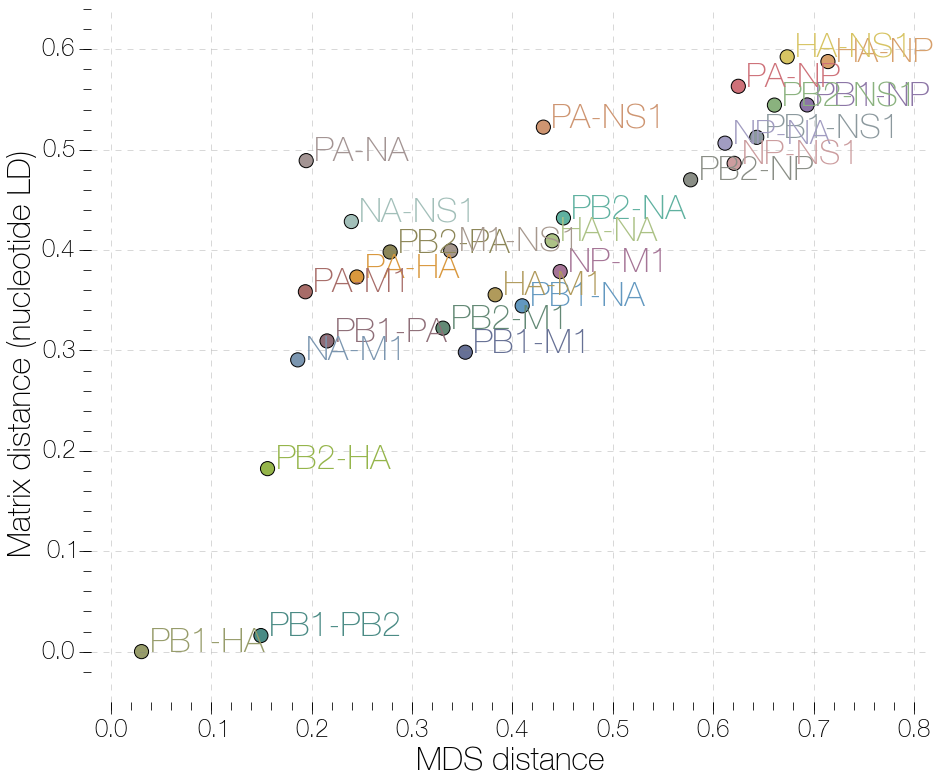
\includegraphics[width=0.65\textwidth]  {supp_figures/InfB_ntLD_MatrixMDScorr.png}
\caption{\textbf{Correlation between mean nucleotide site linkage disequilibrium and MDS embedding distance for all pairs of segments.}}
\label{MDSntCorr}
\end{figure}

\section*{Differences between Vic and Yam PB1-PB2-HA}
Through the combination of inferred PB1-PB2-HA background and realized synonymous and non-synonymous substitution counts on branches \cite{obrien2009} it was possible to investigate whether Victoria and Yamagata lineage backgrounds differ in substitution rates.
Figure \ref{robustCounting} shows the inferred synonymous, non-synonymous (both as substitutions per year) and overall nucleotide substitution rate (as substitutions per site per year) under different lineages of PB1-PB2-HA.

\begin{figure}
\centering  
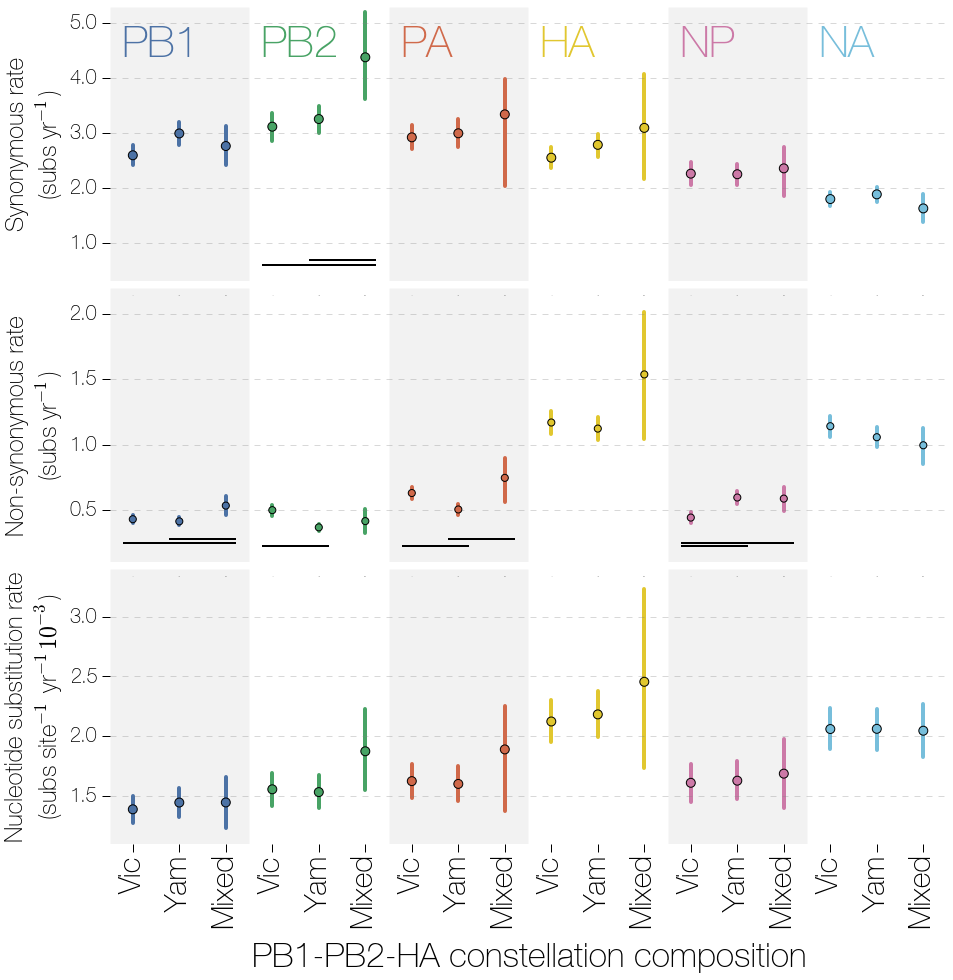
\includegraphics[width=0.65\textwidth]  {supp_figures/InfB_robustCounting.png}
\caption{\textbf{Synonymous, non-synonymous and nucleotide substitution rates in segments under different PB1-PB2-HA complexes.}
Vertical bars indicating uncertainty are 95\% HPDs, black bars indicate 95\% HPDs that do not overlap.}
\label{robustCounting}
\end{figure}

\begin{figure}
\centering  
\includegraphics[width=0.65\textwidth]  {supp_figures/InfB_lineageRatios.png}
\caption{\textbf{Total counts and ratios of Victoria and Yamagata lineage sequences in each segment.}}
\label{lineageRatios}
\end{figure}

\section*{Acknowledgements}
GD was supported by a NERC studentship..... 
TB was supported by a Newton International Fellowship from the Royal Society. 
The research leading to these results has received funding from the European Research Council under the European Community's Seventh Framework Programme (FP7/2007-2013) under Grant Agreement no. 278433-PREDEMICS and ERC Grant agreement no. 260864.
AR and SL acknowledge the support of the Wellcome Trust (grant no. 092807).

\bibliographystyle{pnas}
\bibliography{fluB}
\end{document}